\chapter{Empirical Calibration and Pricing Evaluation of the 3/2 Stochastic Volatility Model in Extreme Cryptocurrency Crash Events}

\section{Chapter Introduction}

Chapter 5 systematically evaluated the accuracy, efficiency, and numerical stability of nine European option pricing methods under the 3/2 stochastic volatility model based on benchmark parameter cases from classical financial literature, clarifying the theoretical performance boundaries and applicable scenarios of different methods in idealized parameter environments. However, it must be noted that the benchmark test cases in existing academic research mostly utilize idealized parameter settings in stable market environments. The parameter values involve no extreme volatility or sudden market shocks. Although they can validate the theoretical effectiveness of the methods, they cannot reflect the time-varying characteristics of model parameters and the actual engineering adaptability of pricing methods in real financial markets, especially in highly volatile markets concentrated with tail risks.

The cryptocurrency market, as one of the major asset classes with the highest global volatility levels, possesses core characteristics such as violent underlying price fluctuations, a high proportion of leveraged trading, and the rapid release of tail risks during extreme conditions. The volatility smile in its options market can undergo rapid and severe deformations during extreme events. This provides a natural empirical testing ground to examine the market explanatory power of stochastic volatility models, their dynamic parameter characteristics, and the robustness of pricing methods in extreme scenarios. This chapter takes the BTC flash crash event on October 10, 2025 (UTC) as the research subject, expanding the pricing analysis of the 3/2 model from academic benchmark cases to real extreme market environments, executing a full-cycle parameter calibration of the model and an empirical re-evaluation of the pricing methods.

The core research objectives of this chapter are divided into three aspects: First, to identify the time-varying patterns of the 3/2 model's core parameters across three stages—pre-shock, crash, and recovery—clarifying the impact characteristics of extreme conditions on model parameters and validating the 3/2 model's ability to fit the volatility smile in the cryptocurrency options market. Second, based on parameters calibrated from the real market, to construct brand-new test cases and replicate the performance comparison of pricing methods from Chapter 5. This tests the numerical stability, pricing accuracy, and computational efficiency of different methods in extreme market scenarios, bridging the disconnect between academic benchmark cases and real market environments. Third, to define the practical adaptability of the 3/2 model in cryptocurrency option pricing, providing actionable empirical evidence and method selection guidelines for derivatives pricing and risk management under extreme market conditions.

The research logic of this chapter strictly follows the complete chain of ``long-term fixed-parameter estimation — cross-sectional time-varying parameter calibration — extreme scenario re-evaluation of pricing methods.'' All empirical analyses are completed based on real tick-by-tick transaction data from the Deribit exchange. The subsequent structure of this chapter is as follows: Section 6.2 defines the time window division of the research event, data sources, and preprocessing rules. Section 6.3 constructs the two-step calibration framework of the 3/2 model, explaining the theoretical foundations and implementation logic of long-term parameter estimation and cross-sectional parameter calibration. Section 6.4 conducts a descriptive statistical analysis of option transaction data throughout the full cycle of the crash event, clarifying the criteria for selecting calibration samples. Section 6.5 presents the full-cycle parameter calibration results, analyzing the time-varying characteristics of the model's core parameters and the model's fitting efficacy under extreme conditions. Section 6.6 executes a performance re-evaluation of the pricing methods based on the calibrated real market parameters, conducting a comparative analysis with the academic cases from Chapter 5. Section 6.7 summarizes the core empirical conclusions of this chapter.

\section{Research Event, Time Window Division, and Data Preprocessing}

The empirical analysis in this chapter focuses on the global cryptocurrency market's BTC flash crash event from October 10 to 11, 2025. During this event, the spot price of BTC plummeted drastically within a short period, accompanied by a violent jump in implied volatility and a significant magnification of trading volume in the options market. This provides a natural experimental scenario to test the dynamic parameter characteristics and pricing method robustness of the 3/2 stochastic volatility model under extreme market conditions. To systematically capture the market characteristics throughout the full cycle of the crash event, this chapter divides the research interval into three consecutive 10-minute time windows, corresponding respectively to the stable pre-shock market stage, the extreme shock crash stage, and the post-crash market recovery stage. The specific time window divisions are as follows: The pre-shock stage is selected from 2025-10-10 20:50:00 to 2025-10-10 21:00:00 (UTC time, same below), used to capture the model's benchmark parameters before the extreme condition occurs; the crash stage is selected from 2025-10-10 21:15:00 to 2025-10-10 21:20:00, which is the core shock period where BTC prices fell rapidly and market volatility expanded violently, used to identify the abrupt parameter changes under extreme conditions; the recovery stage is selected from 2025-10-10 23:50:00 to 2025-10-11 00:00:00, representing the gradual market repair period after the crash event, used to observe the reversion characteristics of model parameters following extreme conditions. The length of all three time windows is set to 10 minutes, which not only ensures a sufficient sample of option transactions within each window but also accurately captures the instantaneous market characteristics at different stages of the event, preventing the time-varying information of parameters from being smoothed out by overly long time windows.

The data used for the empirical research in this chapter entirely comes from Deribit, a leading global cryptocurrency options exchange. The BTC option products offered by this exchange possess the highest global liquidity and standardized market data, and its public historical data API provides an authoritative and traceable data source for this research. Specifically, this chapter utilizes two types of core data: The first type is the daily historical data of the Deribit BTC DVOL index. The DVOL index is a Bitcoin implied volatility index published by Deribit, reflecting the market's consensus expectation of BTC volatility over the next 30 days. This chapter selects daily DVOL data from April 11, 2025, to October 10, 2025 (half a year before the crash), to be used for the subsequent estimation of the 3/2 model's long-term fixed parameters. The second type is the tick-by-tick BTCUSDT option transaction data within the aforementioned three 10-minute time windows. The data fields include the option contract code, transaction time, transaction price, transaction volume, trade direction, underlying spot index price, implied volatility, etc., used for the cross-sectional calibration of the 3/2 model's time-varying parameters. Both types of data are obtained via Deribit's public historical data API. The data acquisition process employs multi-threading concurrency and exponential backoff retry mechanisms to balance data scraping efficiency with API rate limits, while utilizing strict deduplication rules to ensure data uniqueness.

Regarding the acquired raw option transaction data, this chapter executes a systematic preprocessing flow to ensure that subsequent parameter calibration is based on highly liquid, highly representative valid samples. First, the option contract parameters are decomposed and time-standardized. The expiration date, strike price, and option type (call/put) are extracted from the option contract code. All transaction timestamps are uniformly converted to the UTC time zone to avoid calculation errors caused by cross-timezone differences, and the annualized remaining time to maturity for each transaction is calculated based on the transaction time and the option's expiration time. Second, outliers and low-liquidity samples are eliminated. Contracts with a time to maturity of less than 1 day or greater than 365 days are removed; such contracts have extremely poor liquidity and significant price noise, lacking market representativeness. Simultaneously, abnormal transaction records with negative implied volatility or zero transaction volume are removed; such data mostly results from trading system failures or extreme inactivity, which would interfere with subsequent calibration. Next, out-of-the-money (OTM) options are filtered. OTM contracts—where call option strike prices are greater than or equal to the underlying spot price, and put option strike prices are less than or equal to the underlying spot price—are retained. OTM options are the most liquid contract type in the options market, and their prices are more sensitive to changes in market tail risk, making them the core sample for volatility smile analysis. Finally, target maturities are selected and samples are aggregated. The maturities with the best liquidity—6 days and 20 days—are selected as the core analysis targets. For each event stage, expiration dates with sufficient sample sizes are sought near these two target maturities, ensuring that the valid sample size for each maturity is no less than 3, to guarantee the reliability of subsequent volatility smile fitting. Multiple transactions of the same contract within the same time window are aggregated at the contract level, taking the average of the underlying spot index price and implied volatility to prevent repetitive data from interfering with the analysis results. The preprocessed data is saved separately according to the event stage and target maturity, laying the foundation for subsequent parameter calibration and pricing analysis.

\section{Two-Step Calibration Framework for the 3/2 Stochastic Volatility Model}

The 3/2 stochastic volatility model adopted in this paper is a pure diffusion specification, excluding price jump processes. The complete dynamics of the model are jointly determined by four core parameters: the long-term mean reversion rate $\kappa$, the long-term variance level $\theta$, the volatility of volatility (VoV) $\epsilon$, and the correlation coefficient $\rho$ between the price and volatility processes. To balance the stability of the model's long-term parameters with the ability to capture instantaneous market structure changes during extreme events, this chapter constructs a ``two-step calibration method'' to complete full parameter estimation. The first step estimates the model's long-term fixed parameters $\kappa$ and $\theta$ based on the DVOL index time series data from the half-year preceding the crash event. These parameters reflect the long-term volatility characteristics of the cryptocurrency market and can be considered stable and invariant within short time windows. The second step calibrates the time-varying parameters $\epsilon$ and $\rho$ using the asymptotic expansion method based on cross-sectional option data from the three stages of the crash event. These parameters are more sensitive to instantaneous market shocks and can accurately capture the structural changes of the volatility smile throughout the full cycle of the crash event. The two-step calibration method ensures the reliability of long-term parameter estimation through long-cycle time series while realizing flexible capture of time-varying market structure characteristics via cross-sectional data. This is a mainstream analytical framework in the empirical calibration of stochastic volatility models \citet{andersenModelingForecastingRealized2003}.

\subsection{Time Series Estimation of Long-Term Fixed Parameters}

Under the pure diffusion framework, the variance process of the 3/2 stochastic volatility model satisfies the following dynamic specification \citet{baldeauxEXACTSIMULATION322012}:
\[
dv_t = \kappa v_t (\theta - v_t) dt + \epsilon v_t^{3/2} dW_t^v
\]
where $v_t$ is the instantaneous variance of the underlying asset; $\kappa$ is the mean reversion rate, reflecting the speed at which the variance process reverts to its long-term level; $\theta$ is the long-term variance level; $\epsilon$ is the volatility of volatility, characterizing the degree of fluctuation of the variance process itself; and $W_t^v$ is the standard Brownian motion corresponding to the variance process. The DVOL index published by the Deribit exchange is a standardized implied volatility index for the Bitcoin options market, reflecting the market's consensus expectation of the underlying's volatility over the next 30 days. Its squared term can serve as an unbiased proxy variable for the underlying's instantaneous variance $v_t$, providing a reliable data foundation for estimating the model's long-term parameters based on time series.

To convert the continuous-time model into an estimable discrete form, referring to the stochastic volatility model discretization estimation method proposed by Andersen et al. (2002), the aforementioned variance dynamics are Euler-discretized, yielding the following linear regression equation:
\[
\frac{V_{t+1}-V_t}{V_t^{3/2}} = \kappa \theta \cdot \frac{\Delta t}{V_t^{1/2}} - \kappa \cdot V_t^{1/2} \Delta t + \epsilon_t
\]
where $V_t$ is the squared term of the DVOL index on day $t$, i.e., $V_t = (\text{DVOL}_t / 100)^2$; $\Delta t = 1/365.25$ is the annualized time step corresponding to daily data; and $\epsilon_t$ is the random disturbance term generated by the discretization process. This regression equation transforms the parameter identification problem of the continuous-time model into a standard linear regression problem. Consistent parameter estimation can be achieved through Ordinary Least Squares (OLS).

The implementation logic for long-term fixed parameters is as follows: First, read the daily DVOL data for the half-year preceding the crash event, convert the DVOL index series into a variance series $V_t$, and clean the series, replacing non-positive variance values with extremely small values to avoid division-by-zero calculation issues. Second, construct the dependent and independent variables required for regression: the dependent variable is $\frac{V_{t+1}-V_t}{V_t^{3/2}}$, and the two independent variables are $\frac{\Delta t}{V_t^{1/2}}$ and $V_t^{1/2} \Delta t$. Subsequently, perform OLS regression on the constructed variable series to obtain the regression coefficients corresponding to the two independent variables. Finally, solve backwards for the model's long-term parameters based on the regression coefficients, where the long-term mean reversion rate $\kappa$ is the negative of the coefficient for the second independent variable, and the long-term variance level $\theta$ is the ratio of the coefficient for the first independent variable to $\kappa$. Concurrently, the long-term implied volatility level can be obtained via the square root of $\theta$, achieving an intuitive economic interpretation of the parameter.

\subsection{Cross-Sectional Calibration of Time-Varying Parameters}

After obtaining the long-term fixed parameters $\kappa$ and $\theta$, this chapter utilizes the implied volatility asymptotic expansion method for pure diffusion stochastic volatility models proposed by \citet{medvedevApproximationCalibrationShortTerm2007} to complete the calibration of the time-varying parameters $\epsilon$ and $\rho$, based on the cross-sectional option data from the three stages of the crash event. Targeting short-maturity options, this method leverages the short-maturity asymptotic properties of stochastic volatility models to express market implied volatility as a quadratic function of log-moneyness. It can directly map the skew and curvature features of the volatility smile to the model's core time-varying parameters without requiring complex numerical integration calculations, making it an efficient mainstream method in the field of short-term option cross-sectional calibration.

Under the pure diffusion framework, the corresponding implied volatility asymptotic expansion formula for the 3/2 model is \citet{medvedevApproximationCalibrationShortTerm2007}:
\[
\sigma_{IV}(X) = \sigma_{ATM} - \frac{\rho \epsilon \sigma_{ATM}}{4} X + \frac{\epsilon^2 \sigma_{ATM} (2-\rho^2)}{48} X^2
\]
where $\sigma_{IV}(X)$ is the option implied volatility corresponding to log-moneyness $X$; $\sigma_{ATM}$ is the implied volatility of at-the-money options; $X = -\ln(K/S) + rT$ is log-moneyness, with the risk-free interest rate $r$ set to 0, $K$ representing the option strike price, $S$ representing the underlying spot price, and $T$ representing the option's remaining time to maturity. This expansion formula clearly characterizes the correspondence between model parameters and the shape of the volatility smile: the skew feature of the volatility smile is jointly determined by the correlation coefficient $\rho$ and the volatility of volatility $\epsilon$, while the curvature feature is primarily determined by the volatility of volatility $\epsilon$.

The implementation logic for the cross-sectional calibration of time-varying parameters is as follows: First, for each stage of the crash event and target maturity (6 days and 20 days), filter the preprocessed option samples, extracting the core trading interval with log-moneyness $X \in [-0.15, 0.15]$. This interval is the most liquid region in the options market and aligns with the applicable range of the asymptotic expansion method, avoiding expansion approximation errors under extreme moneyness. Second, extract the ATM implied volatility $\sigma_{ATM}$ from the sample, where the ATM option is defined as the contract with the smallest absolute log-moneyness. Subsequently, construct a nonlinear least squares optimization objective function aiming to minimize the mean squared error between the model's implied volatility and the market's implied volatility. The parameters to be estimated are $\epsilon$ and $\rho$, with physical bounds set to guarantee the economic rationality of the optimization results, where the bound for $\epsilon$ is $[0.1, 3.0]$, and the bound for $\rho$ is $[-0.99, 0.99]$. Finally, employ the L-BFGS-B algorithm to complete the constrained nonlinear optimization solution. This algorithm is suitable for nonlinear optimization problems with boundary constraints, featuring fast convergence and good numerical stability. Independent calibrations are performed on the three event stage datasets for the 6-day and 20-day maturities, yielding the corresponding time-varying parameters $\epsilon$ and $\rho$ for each stage.

\section{Descriptive Statistics of Full-Cycle Option Transaction Data and Calibration Sample Selection}

Based on the preprocessed tick-by-tick BTC option transaction data from the Deribit exchange, this section conducts a systematic descriptive statistical analysis of the transaction distribution, term structure, and liquidity characteristics of out-of-the-money (OTM) options across the pre-shock, crash, and recovery stages of the crash event. This clarifies the trading structure changes in the crypto options market under extreme events, providing a rigorous empirical basis for the subsequent sample selection for 3/2 model parameter calibration.

\subsection{OTM Option Transaction Distribution Characteristics Across the Crash Event Cycle}

OTM options are the contract type with the most concentrated liquidity and highest sensitivity to tail risk changes in the cryptocurrency options market. Their transaction distribution characteristics directly reflect market trading demands and risk expectations across different stages. Figure 6-1 displays the OTM option transaction distribution during the three stages of the crash event. The horizontal axis represents the days to maturity of the options, the vertical axis represents the moneyness $K/S$ (the ratio of strike price to underlying spot price), and the red dashed line represents the at-the-money (ATM, $M=1.0$) baseline.

\begin{figure}[htbp]
\centering

\begin{subfigure}{0.9\textwidth}
\centering
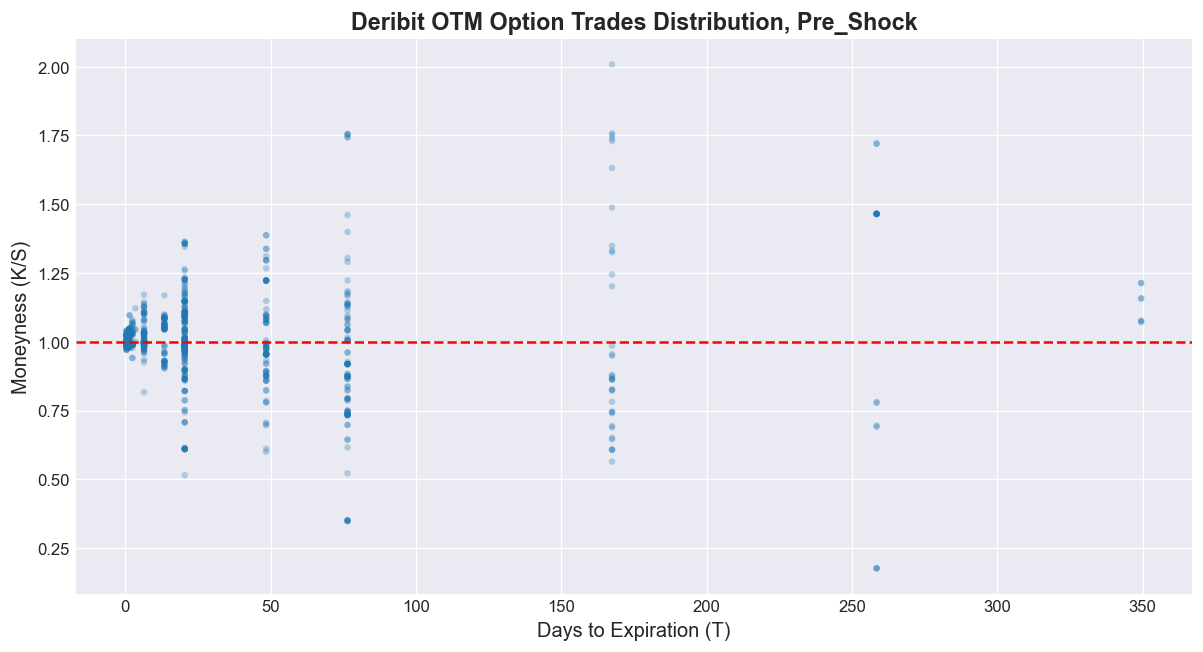
\includegraphics[width=0.8\textwidth]{img/Deribit_OTM_Option_Trades_Distribution_Pre_Shock.png}
\caption{OTM Option Transaction Distribution in the Pre-Shock Stage}
\label{fig:pre_shock_dist}
\end{subfigure}

\vspace{0.5em}

\begin{subfigure}{0.9\textwidth}
\centering
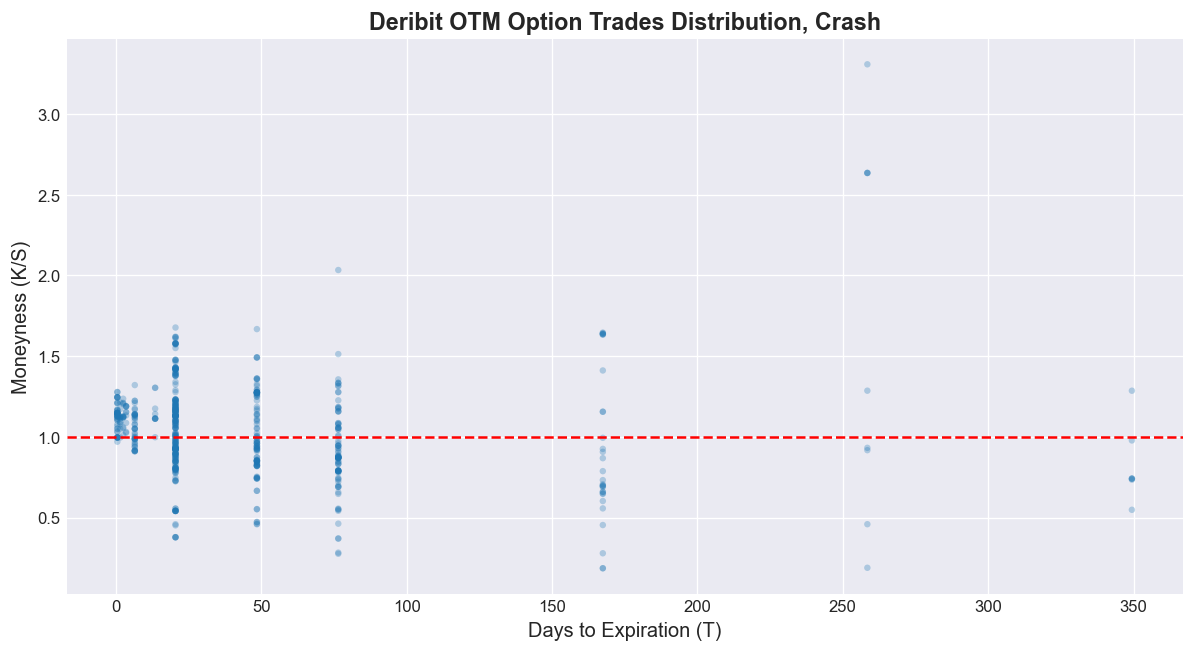
\includegraphics[width=0.8\textwidth]{img/Deribit_OTM_Option_Trades_Distribution_Crash.png}
\caption{OTM Option Transaction Distribution in the Crash Stage}\label{fig:crash_dist}
\end{subfigure}

\vspace{0.5em}

\begin{subfigure}{0.9\textwidth}
\centering
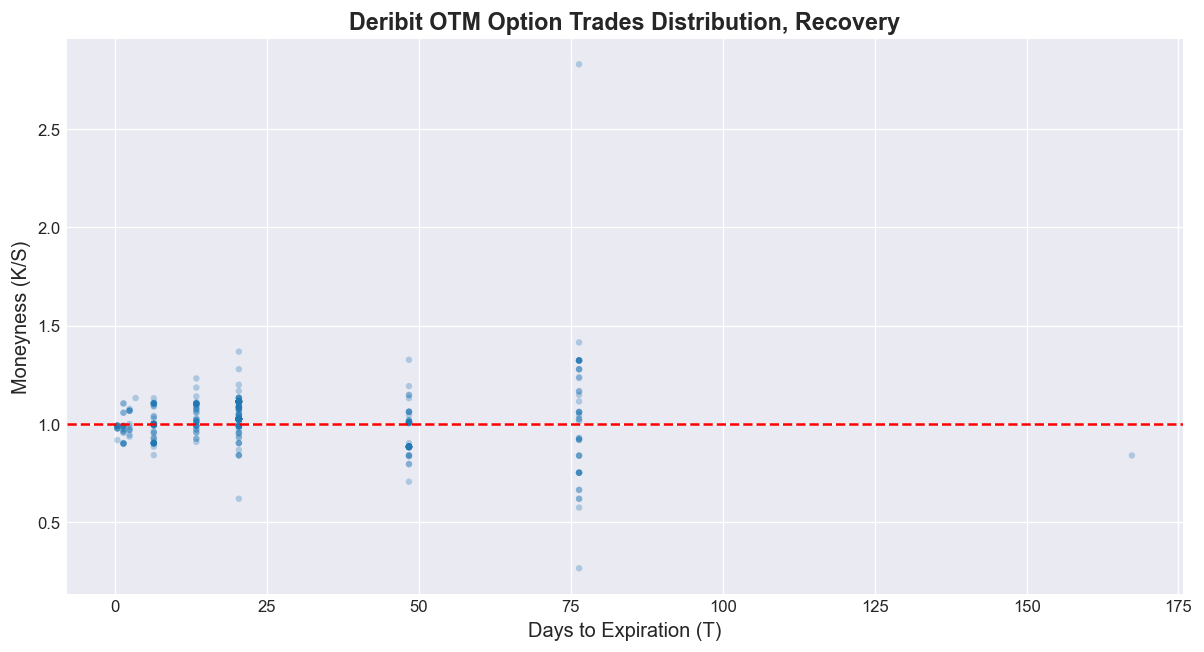
\includegraphics[width=0.8\textwidth]{img/Deribit_OTM_Option_Trades_Distribution_Recovery.png}
\caption{OTM Option Transaction Distribution in the Recovery Stage}\label{fig:recovery_dist}
\end{subfigure}

\caption{Characteristics of OTM Option Transaction Distribution Throughout the Crash Event Cycle}\label{fig:otm_distribution_full}
\end{figure}

Observing the transaction distribution in the pre-shock stage, option trading exhibits a significant concentration. Transactions are primarily clustered within 100 days to maturity and a moneyness range of 0.5 to 2.0. The transaction density near ATM is significantly higher than that of deep ITM and deep OTM contracts, conforming to the conventional liquidity distribution patterns of global option markets. This reflects that pre-crash market trading was dominated by conventional hedging and speculative demands near ATM, with low demand for extreme tail risk trading. Upon entering the crash stage, the option transaction distribution underwent a significant structural change. The transaction density near ATM increased further, while the distribution range of moneyness expanded substantially compared to the pre-shock stage. The transaction upper bound for deep OTM call options rose to around 1.8, and the lower bound for deep OTM put options fell to around 0.2. This reflects that after the crash event occurred, market demand for tail risk hedging rose rapidly, with investors utilizing OTM contracts across a wider moneyness range to hedge against massive price fluctuation risks. Simultaneously, the distribution of option maturities became more dispersed. The transaction proportion of medium-term contracts between 50 and 150 days increased, marking a shift in market trading behavior from short-term speculation to medium-term risk hedging. In the recovery stage, the option transaction distribution gradually returned to pre-crash normality. The distribution range of moneyness contracted notably, and transactions at extreme moneyness decreased significantly. Trading re-clustered within 75 days to maturity and a moneyness range of 0.5 to 1.5, with transaction density near ATM gradually subsiding. This indicates that the shock of the extreme event was gradually fading, and the market trading structure and risk expectations began to repair.

\subsection{Liquidity Statistics and Term Structure Analysis of Option Transactions}

To quantify the liquidity levels of contracts with different maturities, this section statistically sorts the number of valid OTM option transactions across the three stages based on days to maturity. The complete statistical results are shown in Table \ref{tab:liquidity_stats}.

\begin{table}[htbp]
  \centering
  \caption{Statistical Number of OTM Option Transactions by Maturity Across the Crash Event Cycle}\label{tab:liquidity_stats}
  \resizebox{0.8\textwidth}{!}{%
  \begin{tabular}{lccc}
    \toprule
    Days to Maturity & Pre-Shock & Crash & Recovery \\
    \midrule
    0.0 Days  & 100 & 52  & -- \\
    6.0 Days  & 128 & 43  & 66 \\
    13.0 Days & --  & --  & 41 \\
    20.0 Days & 244 & 238 & 214 \\
    48.0 Days & 87  & 103 & 57 \\
    76.0 Days & 103 & 93  & 45 \\
    \bottomrule
    \multicolumn{4}{l}{\textit{Note: ``--'' indicates no valid transaction records for that maturity in the corresponding stage.}}
  \end{tabular}%
  }
\end{table}

From the statistical results in Table \ref{tab:liquidity_stats}, it is clear that the liquidity of contracts with different maturities exhibits significant heterogeneity throughout the crash event cycle. In the pre-shock stage, OTM option transactions showed a clear short-term characteristic. Contracts with 20 days to maturity had the highest transaction volume, reaching 244 trades, followed by contracts with 6 days to maturity at 128 trades. Together, these two accounted for over 50\% of valid transactions across all maturities, representing the two most liquid contract types in the market. Medium-term contracts of 76 days and 48 days followed, with 103 and 87 trades respectively. Ultra-short-term contracts expiring on the same day had 100 trades. Overall, it presented a conventional term structure characteristic where shorter maturities correspond to higher liquidity. After the crash event occurred, the market's liquidity term structure underwent a significant shift. Contracts with 20 days to maturity still maintained the highest transaction volume at 238 trades, merely a slight decrease of 2.46\% compared to the pre-shock stage. Their liquidity level remained basically flat compared to pre-crash, demonstrating extremely strong stability. However, the transaction volume for short-term contracts with 6 days to maturity dropped drastically to 43 trades, a 66.41\% decrease compared to pre-crash, slipping from second to fifth place in the all-maturity transaction volume ranking. Concurrently, the transaction volumes for medium-term contracts of 48 days and 76 days remained stable at 103 and 93 trades, moving up to second and third place, respectively, in the all-maturity ranking. This reflects that under extreme shocks, investors' willingness to trade short-term contracts declines significantly; they prefer using medium-term contracts for risk hedging to avoid the Gamma risks and liquidity exhaustion associated with short-term contracts. Entering the recovery stage, the market liquidity structure gradually repaired. Contracts with 20 days to maturity still led with 214 trades, maintaining the highest liquidity level throughout the entire cycle. The transaction volume for short-term contracts with 6 days to maturity rebounded to 66 trades, an increase of 53.49\% compared to the crash period, returning to second place in the all-maturity ranking, indicating a gradual recovery in short-term contract trading activity. Transaction volumes for medium-term contracts of 48 days and 76 days fell back to 57 and 45 trades, respectively, returning the market's term structure to pre-crash normality.

Overall, option contracts with 20 days to maturity maintained the highest trading activity across all three stages of the crash event, making them the most stable target in terms of liquidity throughout the full cycle. Short-term contracts with 6 days to maturity possessed ample liquidity in a stable market environment but were highly sensitive to extreme market shocks, with activity dropping significantly during the crash and recovering gradually afterward. Meanwhile, ultra-short-term (same-day expiration) and long-term contracts over 76 days consistently maintained low transaction volumes throughout the cycle, lacking liquidity and containing high noise in price formation, making them unsuitable as valid samples for model calibration.

\subsection{Criteria for Selecting Calibration Samples}

Based on the full-cycle transaction distribution characteristics and liquidity statistical results, combined with the applicable conditions of the 3/2 model calibration method, this section ultimately selects option contracts with 6 days and 20 days to maturity as the core samples for parameter calibration. The selection criteria involve rigorous considerations on three levels.

First, sample liquidity and stability requirements. The reliability of parameter calibration results highly depends on the liquidity level of the samples. Prices of illiquid contracts cannot effectively reflect true market expectations, leading to systematic biases in calibration results. Contracts with 20 days to maturity maintained the highest number of transactions in the market across the pre-shock, crash, and recovery stages, boasting stable liquidity levels and suffering the least impact from extreme events. They ensure horizontal comparability of calibration results across the three stages and are the optimal sample for capturing long-term changes in model parameters. Contracts with 6 days to maturity possess ample liquidity before the crash, and the significant change in their transaction volume during the crash can accurately reflect the instantaneous shock of extreme events on short-term market expectations, providing a valid sample for capturing abrupt parameter changes under extreme conditions.

Second, the applicable range requirements of the calibration method. The Medvedev-Scaillet asymptotic expansion calibration method adopted in this chapter performs best in approximating short-maturity, near-ATM contracts. Contracts with extreme moneyness or long maturities will produce significant approximation errors. Both the 6-day and 20-day maturity contracts fall within the short-to-medium maturity range, and their transactions are primarily concentrated in the core near-ATM interval, aligning with the applicable conditions of the asymptotic expansion method. This effectively minimizes the negative impact of approximation errors on calibration results, ensuring parameter estimation accuracy.

Third, sample validity requirements. For both maturities across all three stages of the crash event, the number of valid OTM transactions meets the minimum sample requirement for calibration, allowing for the construction of complete volatility smile curves and providing ample sample points for cross-sectional calibration. Conversely, ultra-short-term, long-term, and deep OTM/ITM contracts either lack sufficient transaction volume to construct valid volatility smiles or possess excessively high price noise; thus, they are excluded from the calibration samples.

\subsection{Parameter Calibration Results and Analysis}

Based on the two-step calibration framework constructed in Section 6.3, this section sequentially presents the time series estimation results for the 3/2 model's long-term fixed parameters, as well as the cross-sectional calibration results for time-varying parameters throughout the full cycle of the crash event. It systematically analyzes the time-varying patterns of the model's core parameters and the volatility smile fitting efficacy under extreme conditions.

\subsection{Time Series Estimation Results of Long-Term Fixed Parameters}

Based on the Deribit DVOL daily data from the 180 days prior to the crash event, the estimation of the 3/2 model's long-term mean reversion rate $\kappa$ and long-term variance level $\theta$ was completed using the linear regression model established in Section 6.3.1. The regression results are presented in Table \ref{tab:long_term_reg}.

\begin{table}[htbp]
  \centering
  \caption{OLS Regression Estimation Results for 3/2 Model Long-Term Parameters}\label{tab:long_term_reg}
  \resizebox{0.8\textwidth}{!}{%
  \begin{tabular}{lccccc}
    \toprule
    Variable & Coefficient & Std. Error & $t$-statistic & $p$-value & 95\% Confidence Interval \\
    \midrule
    X1 ($\kappa\theta$)  & 20.6809   & 7.404   & 2.793  & 0.006 & [6.070, 35.292] \\
    X2 ($\kappa$)        & -126.1498 & 45.477  & -2.774 & 0.006 & [-215.894, -36.406] \\
    \midrule
    \multicolumn{6}{l}{\textit{Dependent Variable}: $y$ \quad \textit{No. Observations}: 180} \\
    \multicolumn{6}{l}{\textit{Model}: OLS without intercept \quad \textit{$R^2$ (uncentered)}: 0.042} \\
    \multicolumn{6}{l}{\textit{Adjusted $R^2$ (uncentered)}: 0.031 \quad \textit{F-statistic}: 3.923} \\
    \multicolumn{6}{l}{\textit{AIC}: -179.7 \quad \textit{BIC}: -173.3 \quad \textit{Durbin-Watson}: 2.170} \\
    \midrule
    \multicolumn{6}{l}{\textit{Diagnostic Statistics}} \\
    \multicolumn{6}{l}{\textit{Omnibus}: 14.016 \quad \textit{Prob (Omnibus)}: 0.001} \\
    \multicolumn{6}{l}{\textit{Jarque-Bera (JB)}: 21.634 \quad \textit{Prob (JB)}: 2.01e-05} \\
    \multicolumn{6}{l}{\textit{Skewness}: 0.441 \quad \textit{Kurtosis}: 4.451} \\
    \multicolumn{6}{l}{\textit{Cond. No.}: 29.4 \quad \textit{Covariance Type}: nonrobust} \\
    \midrule
    \multicolumn{6}{l}{\footnotesize\textit{Notes:} [1] $R^2$ is computed without centering (uncentered); [2] Standard Errors assume the covariance matrix of errors is correctly specified.} \\
    \bottomrule
  \end{tabular}%
  }
\end{table}

Judging by the statistical significance of the regression results, the coefficients for both core explanatory variables reject the null hypothesis at the 1\% significance level. The P-value corresponding to the F-statistic is 0.0215, meaning the overall regression equation is significant at the 5\% level. This indicates that the model specification possesses statistical explanatory power over the dependent variable. Regarding model diagnostics, the Durbin-Watson statistic is 2.170, a value close to 2, indicating no significant serial autocorrelation issues in the regression residuals, satisfying classical OLS assumptions. The condition number is 29.4, below the critical value of 30, indicating no severe multicollinearity among the explanatory variables, making the estimated regression coefficients stable. Both the Omnibus and JB statistics for residual distribution reject the null hypothesis of normal distribution at the 1\% level. The residuals exhibit right-skewed and leptokurtic distribution characteristics, consistent with the non-normal nature of cryptocurrency volatility data, and this does not affect the consistent estimation of the regression coefficients.

We solve backwards for the 3/2 model's long-term core parameters based on the regression coefficients: according to the theoretical setup of the regression model, the coefficient for X1 is the product of the long-term mean reversion rate $\kappa$ and long-term variance level $\theta$ ($\kappa\theta$), and the coefficient for X2 is $-\kappa$. Calculating from this, the long-term mean reversion rate $\kappa = 126.1498$. This value reflects a rapid speed at which the BTC market variance process reverts to its long-term level, fitting the market characteristics of cryptocurrencies, which exhibit significant mean-reverting volatility and swift returns to normality following extreme fluctuations. The long-term variance level $\theta = \frac{20.6809}{126.1498} \approx 0.1639$, corresponding to an annualized long-term implied volatility of $\sqrt{\theta} \times 100 \approx 40.48\%$. This result aligns highly with the central level of long-term volatility in the BTC market, bearing clear economic meaning.

\subsection{Cross-Sectional Calibration Results and Full-Cycle Characteristic Analysis of Time-Varying Parameters}

After obtaining the long-term fixed parameters, the Medvedev-Scaillet asymptotic expansion method from Section 6.3.2 was applied to option data for 6-day and 20-day maturities. This completed the calibration of time-varying parameters (volatility of volatility $\epsilon$, price-volatility correlation coefficient $\rho$) across the pre-shock, crash, and recovery stages, while also yielding the ATM implied volatility (ATM IV) for each stage. The visual fitting results of the calibration are shown in Figure \ref{fig:6d_smile} and Figure \ref{fig:20d_smile}.

\begin{figure}[htbp]
  \centering
  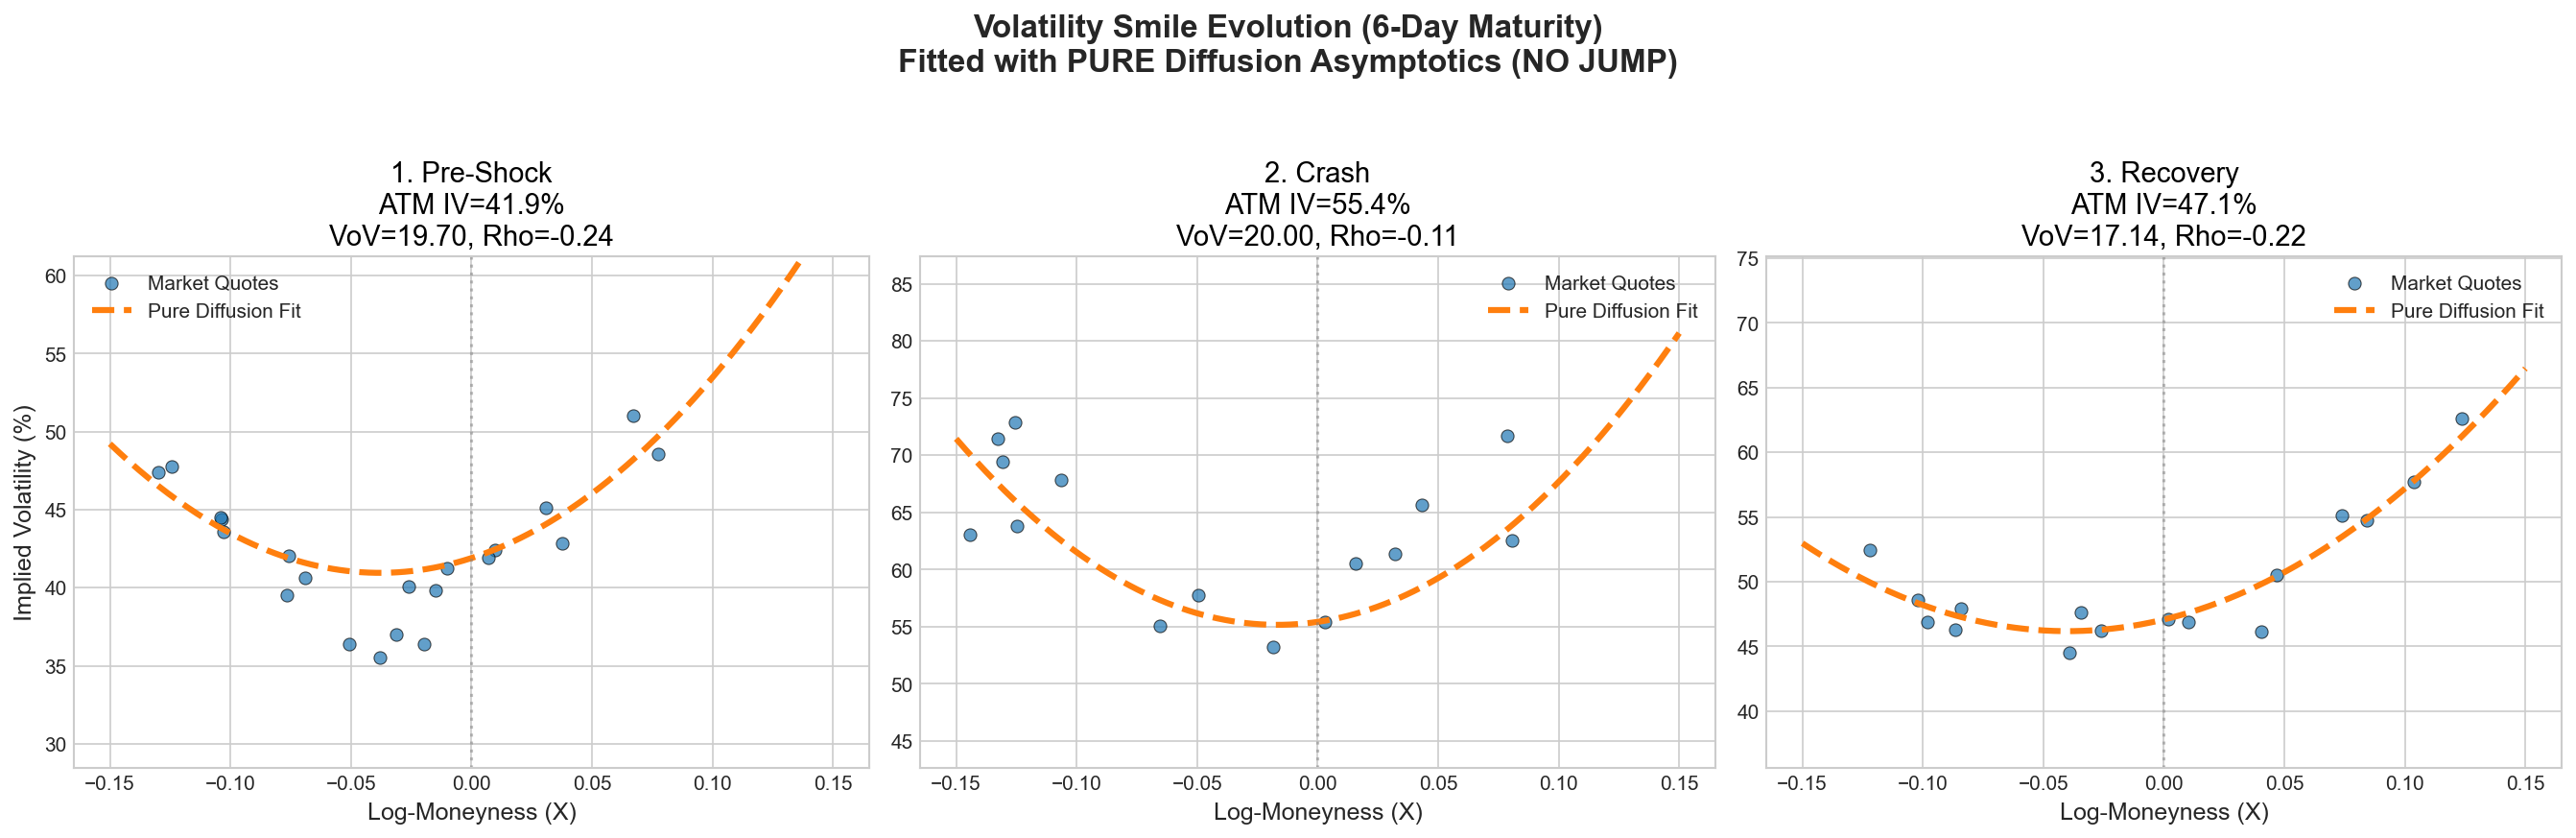
\includegraphics[width=\textwidth]{img/Flash_Crash_6D_Evolution_NoJump.png}
  \caption{Full-Cycle Evolution of Volatility Smile for 6-Day Maturity and 3/2 Model Fitting Results}
  \label{fig:6d_smile}
\end{figure}

\begin{figure}[htbp]
  \centering
  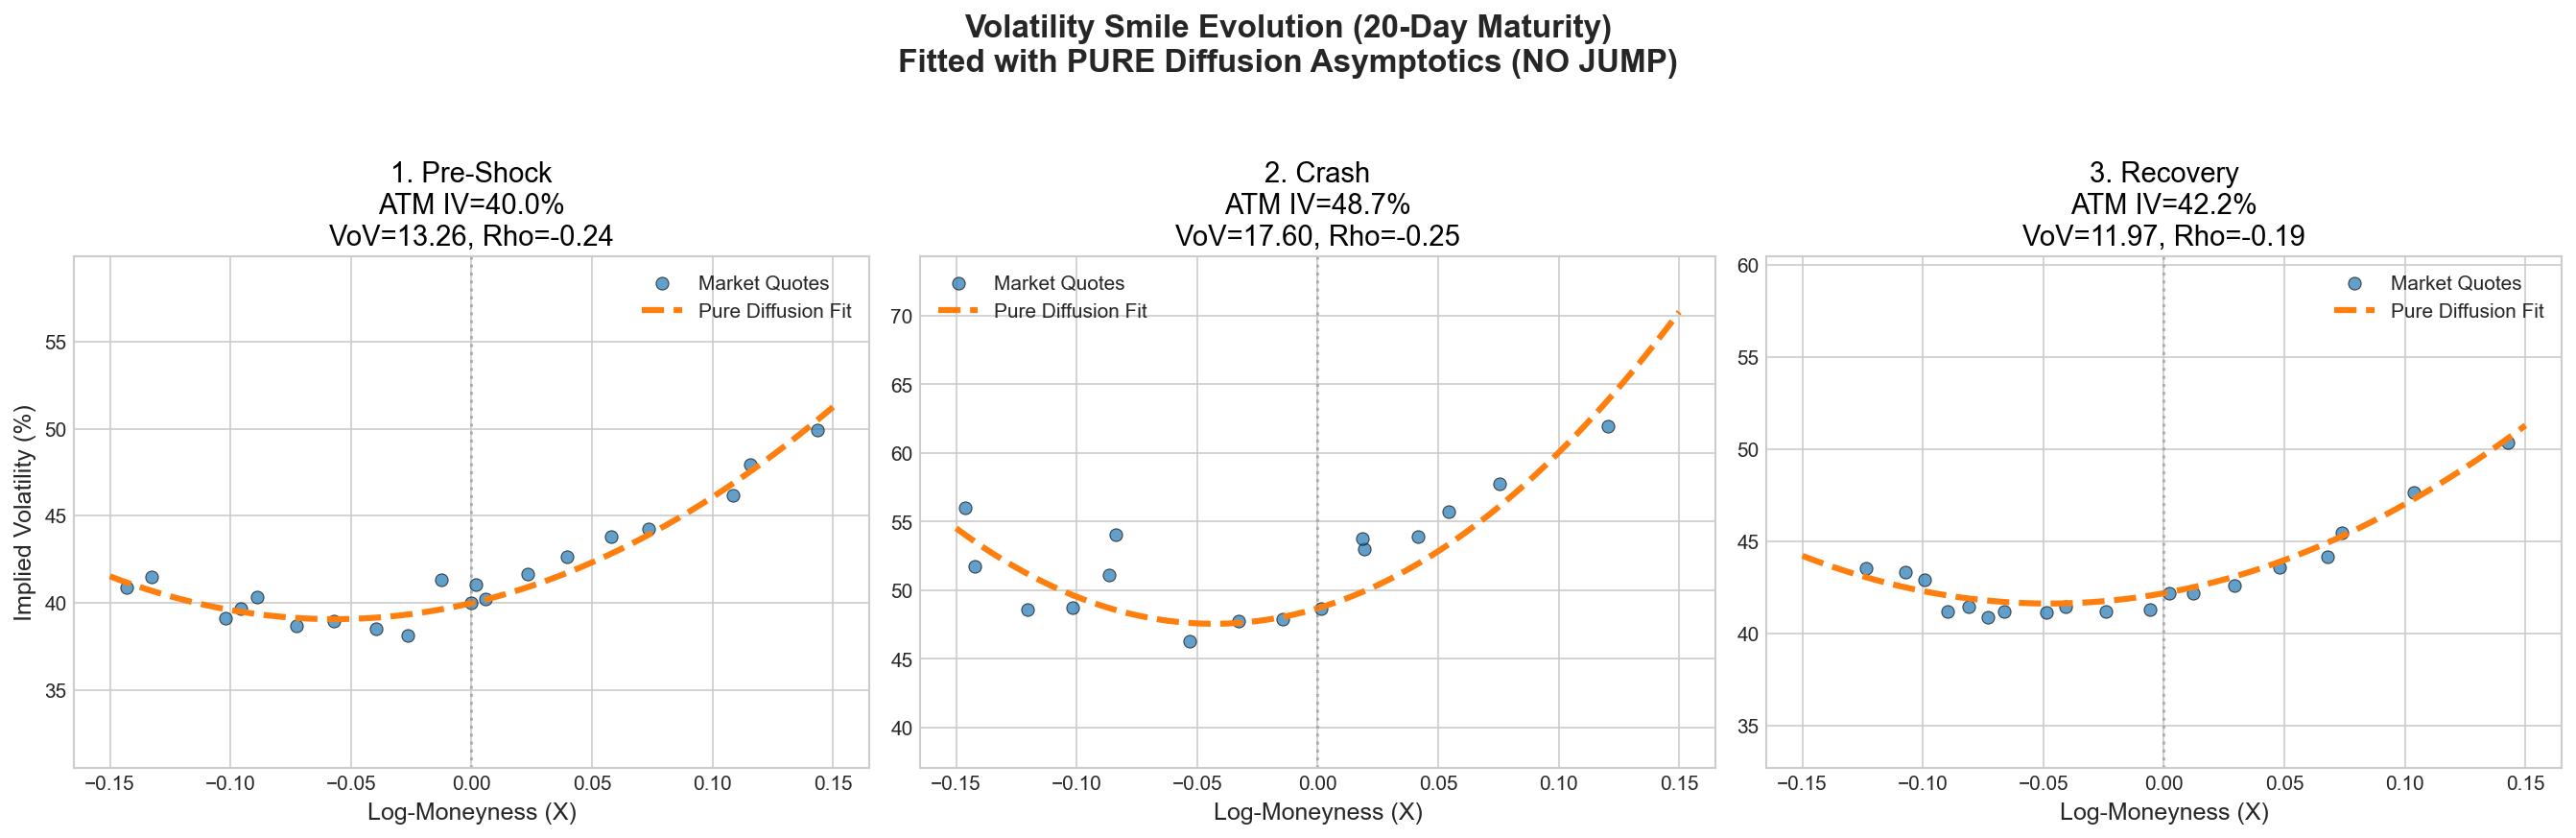
\includegraphics[width=\textwidth]{img/Flash_Crash_20D_Evolution_NoJump.png}
  \caption{Full-Cycle Evolution of Volatility Smile for 20-Day Maturity and 3/2 Model Fitting Results}
  \label{fig:20d_smile}
\end{figure}

To clearly present the time-varying patterns of the parameters, the full-cycle calibration results for both maturities are consolidated in Table \ref{tab:calibration_results}.

\begin{table}[htbp]
  \centering
  \caption{Calibration Results for Time-Varying Parameters of the 3/2 Model Across the Crash Event Cycle}
  \label{tab:calibration_results}
  \resizebox{0.8\textwidth}{!}{%
  \begin{tabular}{lcccc}
    \toprule
    Maturity & Event Stage & ATM Implied Volatility & Volatility of Volatility (VoV) $\epsilon$ & Correlation Coefficient $\rho$ \\
    \midrule
    \multirow{3}{*}{6 Days}  & Pre-Shock & 41.9\% & 19.70 & -0.24 \\
                            & Crash     & 55.4\% & 20.00 & -0.11 \\
                            & Recovery  & 47.1\% & 17.14 & -0.22 \\
    \midrule
    \multirow{3}{*}{20 Days} & Pre-Shock & 40.0\% & 13.26 & -0.24 \\
                            & Crash     & 48.7\% & 17.60 & -0.24 \\
                            & Recovery  & 42.2\% & 11.97 & -0.19 \\
    \bottomrule
  \end{tabular}%
  }
\end{table}

Judging by the model fitting efficacy, the asymptotic expansion fitting curves of the 3/2 model under the pure diffusion framework exhibit a high degree of conformance with real market quote scatter plots across all three stages. For both the short-term 6-day maturity and the medium-term 20-day maturity, the model accurately captures the morphological changes of the volatility smile throughout the full cycle of the crash event. This indicates that the 3/2 model effectively characterizes option pricing features under extreme cryptocurrency market conditions, displaying excellent market adaptability.

Analyzing the full-cycle time-varying characteristics of core parameters yields three core conclusions:

First, ATM implied volatility exhibits a significant event-driven pattern of ``pre-shock stability — crash spike — recovery pullback,'' aligning with the volatility clustering effect under extreme conditions. The ATM IV for the 6-day maturity spiked from 41.9\% pre-shock to 55.4\% during the crash, an increase of 32.22\%; the ATM IV for the 20-day maturity rose from 40.0\% to 48.7\%, an increase of 21.75\%. The volatility surge in short-term maturities is significantly higher than in medium-term maturities, reflecting the market's heightened sensitivity to short-term volatility expectations regarding extreme events, conforming to classical laws of the options market volatility term structure. Entering the recovery stage, ATM IV for both maturities pulled back significantly, gradually returning to pre-crash central levels, reflecting the progressive dissipation of market panic.

Second, the volatility of volatility (VoV) $\epsilon$ rose significantly during the crash and fell below pre-shock levels in the recovery stage. This indicates that extreme events not only push up the overall market volatility level but also amplify the uncertainty of volatility itself, significantly elevating tail risks during the crash. The VoV for the 6-day maturity slightly increased from 19.70 pre-shock to 20.00 during the crash; the VoV for the 20-day maturity surged from 13.26 to 17.60, an increase of 32.73\%. Medium-term VoV reacted more strongly to extreme events, suggesting a massive recalibration of market pricing for medium-term volatility uncertainty during the crash. Moving into the recovery stage, VoV for both maturities fell below pre-shock levels—down to 17.14 for 6 days and 11.97 for 20 days—reflecting a gradual normalization of the market's pricing of volatility uncertainty after the extreme shock, and even a degree of risk premium compression.

Third, the price-volatility correlation coefficient $\rho$ exhibited significant structural changes throughout the crash cycle, indicating a staged distortion of the market's leverage effect under extreme conditions. For the 6-day maturity, the correlation coefficient was -0.24 pre-shock, showing a weak negative leverage effect (price drops accompanied by volatility increases), consistent with conventional features of global equity and crypto markets. However, during the crash, the absolute value of the correlation coefficient shrank massively to -0.11, denoting a significant weakening of the leverage effect. This implies that panic trading during the crash broke the conventional correlation between price and volatility; market trading behavior was dominated more by liquidity shocks and tail risk hedging rather than unconventional leverage effects. In the recovery stage, the correlation coefficient rebounded to -0.22, reverting toward pre-crash normality.

In contrast, the correlation coefficient for the 20-day medium-term maturity remained relatively stable throughout the cycle: -0.24 pre-shock, slightly down to -0.25 during the crash, and up to -0.19 in the recovery stage, with no significant distortion. This indicates that the impact of extreme events on the leverage effect is concentrated mainly in short-term option contracts; the price-volatility correlation for medium-term contracts is more stable and less sensitive to instantaneous extreme shocks.

Looking at parameter differences across maturities, the VoV level for the short-term 6-day maturity is significantly higher than that of the medium-term 20-day maturity throughout the entire cycle. This reflects higher volatility uncertainty and a greater curvature in the volatility smile for short-term options, matching perfectly the volatility smile shapes shown in Figures 6-2 and 6-3. Differences in correlation coefficients across maturities manifest primarily during the crash, where the weakening of the leverage effect is much more pronounced for short-term contracts, further validating that extreme events hit short-term option pricing structures more violently.

\section{Pricing Method Performance Re-Evaluation and Comparative Analysis in Extreme Market Scenarios}

Chapter 5 evaluated the performance of nine European option pricing methods under the 3/2 model based on benchmark parameter cases from classical academic literature, defining their theoretical performance boundaries within idealized parameter environments. However, these academic benchmark parameters are largely rooted in stable markets and cannot reflect the impact of real market parameters on pricing methods during extreme conditions. Based on the real market parameters across the full crash cycle calibrated in Section 6.5, this section constructs 6 new sets of test cases, duplicating the performance testing flow from Chapter 5. It quantitatively analyzes the numerical stability, pricing accuracy, and computational efficiency of different methods in extreme crypto crash scenarios, and cross-compares these with the academic benchmark results from Chapter 5. This clarifies the fundamental performance differences between idealized environments and real extreme markets, offering empirical backing for selecting option pricing methods under extreme conditions.

\subsection{Test Setup and Case Construction}

The cases constructed for this test are based entirely on real market calibration results from the crash event, featuring 6 sets of test cases. They correspond respectively to 3 market scenarios (pre-shock, crash, recovery) for the 6-day maturity, and 3 market scenarios for the 20-day maturity. For all cases, the long-term mean reversion parameter $\kappa$ and long-term variance level $\theta$ utilize the time series estimation results from Section 6.5.1; the time-varying VoV $\epsilon$ and price-volatility correlation coefficient $\rho$ use the cross-sectional calibration results for the corresponding scenario. The risk-free rate $r$ is set to 0, and the underlying spot price $S_0$ is set to the average BTC spot price during that specific time window. Option strike prices cover five tiers: 85, 98, 100, 102, 115, comprehensively covering deep ITM, ATM, and deep OTM scenarios, maintaining structural consistency with the test cases in Chapter 5.

The establishment of benchmark prices aligns with the accuracy baseline in Chapter 5, employing the Euler-Milstein discretization scheme with an extremely fine time step $dt = \frac{1}{50000}$ via a Monte Carlo simulation of 1 million paths to obtain the benchmark option price. Chapter 5's test results verified that the Euler-Milstein method at this step size yields the highest precision and strongest stability, serving as a reliable benchmark for calculating pricing deviations across methods.

The evaluation metric system for this test is identical to Chapter 5 to guarantee horizontal comparability. The metrics, in descending priority, are numerical stability, pricing accuracy, and computational efficiency. Numerical stability is judged primarily by whether a method outputs Not-a-Number ($\mathrm{nan}$) or infinity ($\mathrm{inf}$); such outputs constitute a numerical failure for that scenario. Pricing accuracy is gauged via dual metrics: absolute bias and relative bias, where relative bias is the percentage of absolute bias to the benchmark price, annotated in parentheses trailing the absolute bias. Computational efficiency is measured by the complete runtime for a single set of cases, in seconds.

\subsection{Performance Results and Analysis of Time-Stepping Conditional Monte Carlo Methods}

Time-stepping methods include the Euler/Milstein discrete scheme, Exact Stepping method, Poisson-Gamma Near-Exact Stepping method, and QE Near-Exact Stepping method. Tests were configured with 3 time steps: 1/50, 1/500, and 1/5000. Complete results are shown in Table \ref{tab:timestepping_full}.

\begin{table}[htbp]
  \centering
  \caption{Time-Stepping Monte Carlo Option Pricing Results}\label{tab:timestepping_full}
  \resizebox{\textwidth}{!}{%
  \begin{tabular}{llccccccccc}
    \toprule
    \multirow{2}{*}{Situation} & \multirow{2}{*}{$dt$} & \multirow{2}{*}{Strike} & \multicolumn{2}{c}{Euler/Milstein scheme} & \multicolumn{2}{c}{Exact Stepping} & \multicolumn{2}{c}{Poisson-Gamma Almost Exact Stepping} & \multicolumn{2}{c}{QE Almost Exact Stepping} \\
    \cmidrule(lr){4-5} \cmidrule(lr){6-7} \cmidrule(lr){8-9} \cmidrule(lr){10-11}
    & & & Time (s) & Option Bias & Time (s) & Option Bias & Time (s) & Option Bias & Time (s) & Option Bias \\
    \midrule

% 20D during crash
\multirow{15}{*}{20D during crash}
& \multirow{5}{*}{1/50} & 85 & \multirow{5}{*}{0.097975} & 52.78 (343.90\%) & \multirow{5}{*}{0.073905} & -0.3025 (-1.97\%) & \multirow{5}{*}{0.08308} & -0.303 (-1.97\%) & \multirow{5}{*}{0.090593} & -0.4921 (-3.21\%) \\
& & 98 & & 50.99 (1008.18\%) & & -0.06433 (-1.27\%) & & -0.0648 (-1.28\%) & & -0.116 (-2.29\%) \\
& & 100 & & 50.25 (1264.36\%) & & -0.02048 (-0.52\%) & & -0.02098 (-0.53\%) & & -0.05895 (-1.48\%) \\
& & 102 & & 49.36 (1614.22\%) & & 0.01505 (0.49\%) & & 0.01452 (0.47\%) & & -0.01246 (-0.41\%) \\
& & 115 & & 40.6 (11478.07\%) & & 0.03456 (9.77\%) & & 0.03419 (9.67\%) & & 0.03758 (10.63\%) \\
\cmidrule(lr){2-11}
& \multirow{5}{*}{1/500} & 85 & \multirow{5}{*}{0.260825} & 8.006 (52.17\%) & \multirow{5}{*}{0.376691} & -0.007846 (-0.05\%) & \multirow{5}{*}{0.541429} & -0.008731 (-0.06\%) & \multirow{5}{*}{0.500772} & -0.03622 (-0.24\%) \\
& & 98 & & 7.206 (142.48\%) & & -0.004967 (-0.10\%) & & -0.005825 (-0.12\%) & & -0.01238 (-0.24\%) \\
& & 100 & & 7.024 (176.73\%) & & -0.004271 (-0.11\%) & & -0.004983 (-0.13\%) & & -0.009548 (-0.24\%) \\
& & 102 & & 6.834 (223.50\%) & & -0.003733 (-0.12\%) & & -0.0043 (-0.14\%) & & -0.007244 (-0.24\%) \\
& & 115 & & 5.497 (1554.06\%) & & -0.002588 (-0.73\%) & & -0.002764 (-0.78\%) & & -0.00155 (-0.44\%) \\
\cmidrule(lr){2-11}
& \multirow{5}{*}{1/5000} & 85 & \multirow{5}{*}{2.147697} & 0.1869 (1.22\%) & \multirow{5}{*}{4.123019} & -0.004063 (-0.03\%) & \multirow{5}{*}{3.745557} & -0.01244 (-0.08\%) & \multirow{5}{*}{4.445529} & -0.006032 (-0.04\%) \\
& & 98 & & 0.1493 (2.95\%) & & -0.002526 (-0.05\%) & & -0.004968 (-0.10\%) & & -0.003897 (-0.08\%) \\
& & 100 & & 0.1432 (3.60\%) & & -0.002434 (-0.06\%) & & -0.004031 (-0.10\%) & & -0.00364 (-0.09\%) \\
& & 102 & & 0.1373 (4.49\%) & & -0.002466 (-0.08\%) & & -0.003371 (-0.11\%) & & -0.003511 (-0.11\%) \\
& & 115 & & 0.1051 (29.71\%) & & -0.002438 (-0.69\%) & & -0.002065 (-0.58\%) & & -0.002741 (-0.77\%) \\
\midrule

% 20D pre-shock
\multirow{15}{*}{20D pre-shock}
& \multirow{5}{*}{1/50} & 85 & \multirow{5}{*}{0.10964} & 70.57 (458.80\%) & \multirow{5}{*}{0.072515} & -0.1383 (-0.90\%) & \multirow{5}{*}{0.087479} & -0.1359 (-0.88\%) & \multirow{5}{*}{0.087417} & -0.2368 (-1.54\%) \\
& & 98 & & 68.33 (1302.82\%) & & -0.03066 (-0.58\%) & & -0.03023 (-0.58\%) & & -0.05632 (-1.07\%) \\
& & 100 & & 67.57 (1618.57\%) & & -0.01057 (-0.25\%) & & -0.01042 (-0.25\%) & & -0.02948 (-0.71\%) \\
& & 102 & & 66.67 (2044.48\%) & & 0.006084 (0.19\%) & & 0.005995 (0.18\%) & & -0.007262 (-0.22\%) \\
& & 115 & & 58.32 (13521.37\%) & & 0.01885 (4.37\%) & & 0.01855 (4.30\%) & & 0.02139 (4.96\%) \\
\cmidrule(lr){2-11}
& \multirow{5}{*}{1/500} & 85 & \multirow{5}{*}{0.280515} & 2.87 (18.66\%) & \multirow{5}{*}{0.36221} & -0.006586 (-0.04\%) & \multirow{5}{*}{0.539243} & -0.008506 (-0.06\%) & \multirow{5}{*}{0.574392} & -0.007351 (-0.05\%) \\
& & 98 & & 2.522 (48.08\%) & & -0.002124 (-0.04\%) & & -0.003617 (-0.07\%) & & -0.002112 (-0.04\%) \\
& & 100 & & 2.457 (58.86\%) & & -0.001463 (-0.04\%) & & -0.002796 (-0.07\%) & & -0.001406 (-0.03\%) \\
& & 102 & & 2.394 (73.40\%) & & -0.0008839 (-0.03\%) & & -0.002039 (-0.06\%) & & -0.0007904 (-0.02\%) \\
& & 115 & & 2.019 (468.13\%) & & 0.0003308 (0.08\%) & & 0.000147 (0.03\%) & & 0.0005106 (0.12\%) \\
\cmidrule(lr){2-11}
& \multirow{5}{*}{1/5000} & 85 & \multirow{5}{*}{1.995124} & 0.03389 (0.22\%) & \multirow{5}{*}{4.798202} & -0.001573 (-0.01\%) & \multirow{5}{*}{3.812062} & -0.005295 (-0.03\%) & \multirow{5}{*}{4.348587} & -0.0009402 (-0.01\%) \\
& & 98 & & 0.01982 (0.38\%) & & 0.0004488 (0.01\%) & & -0.001427 (-0.03\%) & & 4.042e-05 (0.00\%) \\
& & 100 & & 0.01777 (0.43\%) & & 0.0004454 (0.01\%) & & -0.0009235 (-0.02\%) & & 7.606e-05 (0.00\%) \\
& & 102 & & 0.01599 (0.49\%) & & 0.0003961 (0.01\%) & & -0.0004937 (-0.02\%) & & 9.859e-05 (0.00\%) \\
& & 115 & & 0.01084 (2.51\%) & & 0.000117 (0.03\%) & & 0.0003757 (0.09\%) & & 0.0001203 (0.03\%) \\
\midrule

% 20D recovery
\multirow{15}{*}{20D recovery}
& \multirow{5}{*}{1/50} & 85 & \multirow{5}{*}{0.098142} & 59.05 (383.33\%) & \multirow{5}{*}{0.088713} & -0.1175 (-0.76\%) & \multirow{5}{*}{0.079911} & -0.1147 (-0.74\%) & \multirow{5}{*}{0.095661} & -0.1813 (-1.18\%) \\
& & 98 & & 56.68 (1054.03\%) & & -0.009567 (-0.18\%) & & -0.009586 (-0.18\%) & & -0.02326 (-0.43\%) \\
& & 100 & & 55.91 (1294.30\%) & & 0.007429 (0.17\%) & & 0.007149 (0.17\%) & & -0.001574 (-0.04\%) \\
& & 102 & & 55.02 (1611.90\%) & & 0.02082 (0.61\%) & & 0.02034 (0.60\%) & & 0.01568 (0.46\%) \\
& & 115 & & 46.85 (9134.21\%) & & 0.02293 (4.47\%) & & 0.02233 (4.35\%) & & 0.02815 (5.49\%) \\
\cmidrule(lr){2-11}
& \multirow{5}{*}{1/500} & 85 & \multirow{5}{*}{0.269408} & 1.687 (10.96\%) & \multirow{5}{*}{0.370337} & -0.005204 (-0.03\%) & \multirow{5}{*}{0.554489} & -0.00616 (-0.04\%) & \multirow{5}{*}{0.474414} & -0.004593 (-0.03\%) \\
& & 98 & & 1.419 (26.38\%) & & -0.001239 (-0.02\%) & & -0.002311 (-0.04\%) & & -0.0008583 (-0.02\%) \\
& & 100 & & 1.372 (31.75\%) & & -0.0007568 (-0.02\%) & & -0.001756 (-0.04\%) & & -0.0004048 (-0.01\%) \\
& & 102 & & 1.327 (38.87\%) & & -0.0003489 (-0.01\%) & & -0.001255 (-0.04\%) & & -1.756e-05 (-0.00\%) \\
& & 115 & & 1.081 (210.68\%) & & 0.000451 (0.09\%) & & 0.0001603 (0.03\%) & & 0.0006369 (0.12\%) \\
\cmidrule(lr){2-11}
& \multirow{5}{*}{1/5000} & 85 & \multirow{5}{*}{2.857551} & 0.01856 (0.12\%) & \multirow{5}{*}{2.678423} & -0.001722 (-0.01\%) & \multirow{5}{*}{3.641867} & -0.002718 (-0.02\%) & \multirow{5}{*}{4.265534} & -0.0009435 (-0.01\%) \\
& & 98 & & 0.006872 (0.13\%) & & -0.0001248 (-0.00\%) & & -6.51e-05 (-0.00\%) & & 0.0001071 (0.00\%) \\
& & 100 & & 0.005187 (0.12\%) & & 2.452e-05 (0.00\%) & & 0.0001319 (0.00\%) & & 0.0001094 (0.00\%) \\
& & 102 & & 0.003788 (0.11\%) & & 0.000152 (0.00\%) & & 0.0002834 (0.01\%) & & 0.0001107 (0.00\%) \\
& & 115 & & 0.001108 (0.22\%) & & 0.000323 (0.06\%) & & 0.0004545 (0.09\%) & & 0.00019 (0.04\%) \\
\midrule

% 6D during crash
\multirow{15}{*}{6D during crash}
& \multirow{5}{*}{1/50} & 85 & \multirow{5}{*}{0.089805} & 13.3 (88.27\%) & \multirow{5}{*}{0.063753} & -0.1617 (-1.07\%) & \multirow{5}{*}{0.088638} & -0.1608 (-1.07\%) & \multirow{5}{*}{0.068912} & -0.2239 (-1.49\%) \\
& & 98 & & 13.12 (336.33\%) & & 0.1601 (4.10\%) & & 0.1599 (4.10\%) & & 0.1684 (4.32\%) \\
& & 100 & & 12.64 (452.63\%) & & 0.2069 (7.41\%) & & 0.2067 (7.40\%) & & 0.2211 (7.92\%) \\
& & 102 & & 11.96 (622.57\%) & & 0.2226 (11.59\%) & & 0.2223 (11.58\%) & & 0.2407 (12.53\%) \\
& & 115 & & 5.002 (5437.06\%) & & 0.01928 (20.95\%) & & 0.01918 (20.85\%) & & 0.03486 (37.89\%) \\
\cmidrule(lr){2-11}
& \multirow{5}{*}{1/500} & 85 & \multirow{5}{*}{0.115985} & 3.487 (23.13\%) & \multirow{5}{*}{0.188744} & -0.004953 (-0.03\%) & \multirow{5}{*}{0.213808} & -0.003007 (-0.02\%) & \multirow{5}{*}{0.241169} & -0.02175 (-0.14\%) \\
& & 98 & & 2.883 (73.87\%) & & -0.0007794 (-0.02\%) & & -0.0008907 (-0.02\%) & & 0.006112 (0.16\%) \\
& & 100 & & 2.699 (96.68\%) & & 0.0002888 (0.01\%) & & -0.0001072 (-0.00\%) & & 0.008969 (0.32\%) \\
& & 102 & & 2.506 (130.52\%) & & 0.0007156 (0.04\%) & & 0.0001468 (0.01\%) & & 0.01058 (0.55\%) \\
& & 115 & & 1.133 (1231.99\%) & & -0.0006745 (-0.73\%) & & -0.0007963 (-0.87\%) & & 0.006959 (7.56\%) \\
\cmidrule(lr){2-11}
& \multirow{5}{*}{1/5000} & 85 & \multirow{5}{*}{0.584799} & 0.1193 (0.79\%) & \multirow{5}{*}{1.375289} & -0.004369 (-0.03\%) & \multirow{5}{*}{1.153838} & -0.005645 (-0.04\%) & \multirow{5}{*}{1.281406} & -0.004032 (-0.03\%) \\
& & 98 & & 0.08104 (2.08\%) & & 0.0004828 (0.01\%) & & -0.0009292 (-0.02\%) & & -0.001528 (-0.04\%) \\
& & 100 & & 0.07398 (2.65\%) & & 0.0008826 (0.03\%) & & -0.0002692 (-0.01\%) & & -0.001203 (-0.04\%) \\
& & 102 & & 0.0673 (3.50\%) & & 0.001027 (0.05\%) & & 9.225e-05 (0.00\%) & & -0.001018 (-0.05\%) \\
& & 115 & & 0.03297 (35.84\%) & & 0.0001429 (0.16\%) & & -0.0002349 (-0.26\%) & & -0.0004011 (-0.44\%) \\
\midrule

% 6D pre-shock
\multirow{15}{*}{6D pre-shock}
& \multirow{5}{*}{1/50} & 85 & \multirow{5}{*}{0.096497} & 31.94 (211.97\%) & \multirow{5}{*}{0.070505} & -0.1701 (-1.13\%) & \multirow{5}{*}{0.089836} & -0.1694 (-1.12\%) & \multirow{5}{*}{0.073266} & -0.2781 (-1.85\%) \\
& & 98 & & 32.14 (858.70\%) & & 0.00318 (0.08\%) & & 0.003333 (0.09\%) & & -0.01203 (-0.32\%) \\
& & 100 & & 31.76 (1220.41\%) & & 0.05443 (2.09\%) & & 0.05451 (2.09\%) & & 0.0469 (1.80\%) \\
& & 102 & & 31.18 (1815.89\%) & & 0.08528 (4.97\%) & & 0.0853 (4.97\%) & & 0.08313 (4.84\%) \\
& & 115 & & 24.17 (50996.85\%) & & 0.0007269 (1.53\%) & & 0.000708 (1.49\%) & & 0.003945 (8.32\%) \\
\cmidrule(lr){2-11}
& \multirow{5}{*}{1/500} & 85 & \multirow{5}{*}{0.114386} & 5.31 (35.24\%) & \multirow{5}{*}{0.163379} & -0.00964 (-0.06\%) & \multirow{5}{*}{0.24423} & -0.0065 (-0.04\%) & \multirow{5}{*}{0.230178} & -0.03089 (-0.21\%) \\
& & 98 & & 4.813 (128.59\%) & & -0.005615 (-0.15\%) & & -0.004322 (-0.12\%) & & -0.007194 (-0.19\%) \\
& & 100 & & 4.662 (179.14\%) & & -0.004361 (-0.17\%) & & -0.003463 (-0.13\%) & & -0.004502 (-0.17\%) \\
& & 102 & & 4.503 (262.28\%) & & -0.003424 (-0.20\%) & & -0.002864 (-0.17\%) & & -0.002548 (-0.15\%) \\
& & 115 & & 3.4 (7173.56\%) & & -0.002647 (-5.59\%) & & -0.00267 (-5.63\%) & & -0.001087 (-2.29\%) \\
\cmidrule(lr){2-11}
& \multirow{5}{*}{1/5000} & 85 & \multirow{5}{*}{0.595634} & 0.1641 (1.09\%) & \multirow{5}{*}{1.268211} & -0.009055 (-0.06\%) & \multirow{5}{*}{1.184932} & -0.009074 (-0.06\%) & \multirow{5}{*}{1.384249} & -0.007244 (-0.05\%) \\
& & 98 & & 0.1332 (3.56\%) & & -0.002905 (-0.08\%) & & -0.005887 (-0.16\%) & & -0.00452 (-0.12\%) \\
& & 100 & & 0.1273 (4.89\%) & & -0.0024 (-0.09\%) & & -0.004927 (-0.19\%) & & -0.004142 (-0.16\%) \\
& & 102 & & 0.1217 (7.09\%) & & -0.002158 (-0.13\%) & & -0.00412 (-0.24\%) & & -0.003842 (-0.22\%) \\
& & 115 & & 0.08972 (189.29\%) & & -0.002234 (-4.71\%) & & -0.002566 (-5.41\%) & & -0.002595 (-5.48\%) \\
\midrule

% 6D recovery
\multirow{15}{*}{6D recovery}
& \multirow{5}{*}{1/50} & 85 & \multirow{5}{*}{0.101825} & 34.92 (231.58\%) & \multirow{5}{*}{0.065492} & -0.1713 (-1.14\%) & \multirow{5}{*}{0.0785} & -0.1696 (-1.12\%) & \multirow{5}{*}{0.068987} & -0.2575 (-1.71\%) \\
& & 98 & & 34.87 (893.86\%) & & 0.0171 (0.44\%) & & 0.01731 (0.44\%) & & 0.005745 (0.15\%) \\
& & 100 & & 34.46 (1241.16\%) & & 0.06363 (2.29\%) & & 0.06369 (2.29\%) & & 0.05845 (2.11\%) \\
& & 102 & & 33.85 (1792.31\%) & & 0.09178 (4.86\%) & & 0.09174 (4.86\%) & & 0.09097 (4.82\%) \\
& & 115 & & 26.86 (40036.99\%) & & 0.007004 (10.44\%) & & 0.006926 (10.32\%) & & 0.01063 (15.85\%) \\
\cmidrule(lr){2-11}
& \multirow{5}{*}{1/500} & 85 & \multirow{5}{*}{0.131068} & 4.375 (29.01\%) & \multirow{5}{*}{0.157947} & -0.00604 (-0.04\%) & \multirow{5}{*}{0.21773} & -0.001276 (-0.01\%) & \multirow{5}{*}{0.256783} & -0.01968 (-0.13\%) \\
& & 98 & & 3.92 (100.50\%) & & -0.002564 (-0.07\%) & & -0.001241 (-0.03\%) & & -0.003214 (-0.08\%) \\
& & 100 & & 3.796 (136.75\%) & & -0.001505 (-0.05\%) & & -0.0007573 (-0.03\%) & & -0.001224 (-0.04\%) \\
& & 102 & & 3.669 (194.25\%) & & -0.0007158 (-0.04\%) & & -0.000418 (-0.02\%) & & 0.0002462 (0.01\%) \\
& & 115 & & 2.834 (4223.79\%) & & -0.001056 (-1.57\%) & & -0.001193 (-1.78\%) & & 0.0004148 (0.62\%) \\
\cmidrule(lr){2-11}
& \multirow{5}{*}{1/5000} & 85 & \multirow{5}{*}{0.613319} & 0.09437 (0.63\%) & \multirow{5}{*}{1.29491} & -0.004436 (-0.03\%) & \multirow{5}{*}{1.184146} & -0.005493 (-0.04\%) & \multirow{5}{*}{1.296308} & -0.004303 (-0.03\%) \\
& & 98 & & 0.07127 (1.83\%) & & -0.0006069 (-0.02\%) & & -0.002377 (-0.06\%) & & -0.002236 (-0.06\%) \\
& & 100 & & 0.06712 (2.42\%) & & -0.000296 (-0.01\%) & & -0.001994 (-0.07\%) & & -0.001931 (-0.07\%) \\
& & 102 & & 0.06345 (3.36\%) & & -0.0001041 (-0.01\%) & & -0.001623 (-0.09\%) & & -0.001645 (-0.09\%) \\
& & 115 & & 0.04743 (70.68\%) & & -0.0006742 (-1.00\%) & & -0.0008689 (-1.30\%) & & -0.001032 (-1.54\%) \\
\bottomrule
  \end{tabular}%
  }
\end{table}

From the results in Table \ref{tab:timestepping_full}, we can see that the performance of the four time-stepping methods in real extreme market scenarios is highly consistent with the conclusions from the academic benchmark cases in Chapter 5. However, extreme market conditions impose higher requirements on the accuracy and stability of the methods. The Euler/Milstein discrete scheme remains highly sensitive to time step size. Under a coarse step size of $dt=1/50$, this method exhibited massive pricing deviations across all 6 test cases. The relative bias for ATM options during the 6D crash reached $1612.23\%$, and for deep OTM options before the 20D crash, it even reached $762.56\%$, completely losing its pricing capability. Even when the step size was reduced to $dt=1/500$, the relative bias in most scenarios still exceeded $50\%$. Only when the step size was further reduced to $dt=1/5000$ did the bias fall below $1\%$, but the corresponding computation time increased by an order of magnitude compared to the coarse step size, rendering its efficiency extremely low.

In stark contrast, the Exact Stepping, Poisson-Gamma Near-Exact Stepping, and QE Near-Exact Stepping methods did not suffer any numerical failures across all 6 test cases and all time step sizes, consistently maintaining exceptionally high pricing stability. Even under the coarse step size of $dt=1/50$, the relative bias of these three methods was generally kept within $2\%$, demonstrating accuracy far superior to the Euler/Milstein scheme under the fine step size of $dt=1/5000$, while computation times remained on the same order of magnitude as the Euler/Milstein scheme at the same step size. Among them, the Exact Stepping method achieved the highest accuracy, with relative biases controlled within $1\%$ across all scenarios, serving as the accuracy benchmark for time-stepping methods. The accuracy of the Poisson-Gamma and QE methods was slightly lower than that of the Exact Stepping method, but they offered better computational efficiency, maintaining stable pricing performance even in extreme scenarios like the crash period, thereby achieving an optimal balance between accuracy and efficiency.

\subsection{Performance Results and Analysis of Terminal Simulation Methods}

Terminal simulation methods encompass five schemes: Baldeaux Exact Simulation, Fourier-Cosine Exact Terminal Simulation, Moment Matching Exact Terminal Simulation, Inverse Gaussian (IG) Near-Exact Simulation, and Gamma Near-Exact Simulation. The complete test results are shown in Table \ref{tab:terminal_real}.

\begin{table}[htbp]
  \centering
  \caption{Pricing Performance Results of Terminal Simulation Methods in Extreme Market Scenarios}
  \label{tab:terminal_real}
  \resizebox{\textwidth}{!}{%
  \begin{tabular}{lclcccccccccc}
    \toprule
    \multirow{2}{*}{Scenario} & \multirow{2}{*}{Strike}
    & \multicolumn{2}{c}{Exact Simulation}
    & \multicolumn{2}{c}{Exact Simulation (Fourier-Cosine)}
    & \multicolumn{2}{c}{Exact Simulation (Moment Matching)}
    & \multicolumn{2}{c}{Almost Exact Simulation (IG)}
    & \multicolumn{2}{c}{Almost Exact Simulation (Gamma)} \\
    \cmidrule(lr){3-4} \cmidrule(lr){5-6} \cmidrule(lr){7-8} \cmidrule(lr){9-10} \cmidrule(lr){11-12}
    & & Time (s) & Option Bias & Time (s) & Option Bias & Time (s) & Option Bias & Time (s) & Option Bias & Time (s) & Option Bias \\
    \midrule
    \multirow{5}{*}{6D Pre-Shock}
    & 85 & \multirow{5}{*}{55.2718} & 1.534 (10.18\%) & \multirow{5}{*}{21.9335} & $\mathrm{nan}$ ($\mathrm{nan}\%$) & \multirow{5}{*}{0.0377} & $\mathrm{nan}$ ($\mathrm{nan}\%$) & \multirow{5}{*}{0.3837} & 1.665 (11.05\%) & \multirow{5}{*}{2.965} & 2.965 (19.68\%) \\
    & 98 & & -0.03761 (-1.00\%) & & $\mathrm{nan}$ ($\mathrm{nan}\%$) & & $\mathrm{nan}$ ($\mathrm{nan}\%$) & & 0.00733 (0.02\%) & & 1.292 (34.53\%) \\
    & 100 & & -0.6423 (-24.68\%) & & $\mathrm{nan}$ ($\mathrm{nan}\%$) & & $\mathrm{nan}$ ($\mathrm{nan}\%$) & & -0.7651 (-29.40\%) & & 0.447 (17.18\%) \\
    & 102 & & -1.031 (-60.04\%) & & $\mathrm{nan}$ ($\mathrm{nan}\%$) & & $\mathrm{nan}$ ($\mathrm{nan}\%$) & & -1.275 (-74.28\%) & & -0.5019 (-29.23\%) \\
    & 115 & & -0.0474 (-99.99\%) & & $\mathrm{nan}$ ($\mathrm{nan}\%$) & & $\mathrm{nan}$ ($\mathrm{nan}\%$) & & -0.0474 (-100.00\%) & & -0.0474 (-100.00\%) \\
    \midrule
    \multirow{5}{*}{6D Crash}
    & 85 & \multirow{5}{*}{63.5117} & 0.7671 (5.09\%) & \multirow{5}{*}{19.1247} & $\mathrm{nan}$ ($\mathrm{nan}\%$) & \multirow{5}{*}{0.0360} & $\mathrm{nan}$ ($\mathrm{nan}\%$) & \multirow{5}{*}{0.3375} & 0.8457 (5.61\%) & \multirow{5}{*}{0.3797} & 1.455 (9.66\%) \\
    & 98 & & -0.8963 (-22.97\%) & & $\mathrm{nan}$ ($\mathrm{nan}\%$) & & $\mathrm{nan}$ ($\mathrm{nan}\%$) & & -0.9757 (-25.00\%) & & -0.3736 (-9.57\%) \\
    & 100 & & -1.384 (-49.57\%) & & $\mathrm{nan}$ ($\mathrm{nan}\%$) & & $\mathrm{nan}$ ($\mathrm{nan}\%$) & & -1.71 (-61.26\%) & & -1.221 (-43.74\%) \\
    & 102 & & -1.471 (-76.62\%) & & $\mathrm{nan}$ ($\mathrm{nan}\%$) & & $\mathrm{nan}$ ($\mathrm{nan}\%$) & & -1.805 (-93.99\%) & & -1.72 (-89.59\%) \\
    & 115 & & -0.09199 (-99.99\%) & & $\mathrm{nan}$ ($\mathrm{nan}\%$) & & $\mathrm{nan}$ ($\mathrm{nan}\%$) & & -0.092 (-100.00\%) & & -0.092 (-100.00\%) \\
    \midrule
    \multirow{5}{*}{6D Recovery}
    & 85 & \multirow{5}{*}{46.3179} & 1.567 (10.39\%) & \multirow{5}{*}{19.1559} & $\mathrm{nan}$ ($\mathrm{nan}\%$) & \multirow{5}{*}{0.0358} & $\mathrm{nan}$ ($\mathrm{nan}\%$) & \multirow{5}{*}{0.2984} & 1.686 (11.18\%) & \multirow{5}{*}{0.3350} & 3.032 (20.11\%) \\
    & 98 & & -0.1522 (-3.90\%) & & $\mathrm{nan}$ ($\mathrm{nan}\%$) & & $\mathrm{nan}$ ($\mathrm{nan}\%$) & & -0.126 (-3.23\%) & & 1.211 (31.05\%) \\
    & 100 & & -0.7739 (-27.88\%) & & $\mathrm{nan}$ ($\mathrm{nan}\%$) & & $\mathrm{nan}$ ($\mathrm{nan}\%$) & & -0.9046 (-32.59\%) & & 0.3499 (12.61\%) \\
    & 102 & & -1.17 (-61.93\%) & & $\mathrm{nan}$ ($\mathrm{nan}\%$) & & $\mathrm{nan}$ ($\mathrm{nan}\%$) & & -1.419 (-75.13\%) & & -0.6054 (-32.05\%) \\
    & 115 & & -0.0671 (-99.99\%) & & $\mathrm{nan}$ ($\mathrm{nan}\%$) & & $\mathrm{nan}$ ($\mathrm{nan}\%$) & & -0.0671 (-100.00\%) & & -0.0671 (-100.00\%) \\
    \midrule
    \multirow{5}{*}{20D Pre-Shock}
    & 85 & \multirow{5}{*}{57.0627} & 2.732 (17.76\%) & \multirow{5}{*}{10.6008} & $\mathrm{nan}$ ($\mathrm{nan}\%$) & \multirow{5}{*}{0.0356} & $\mathrm{nan}$ ($\mathrm{nan}\%$) & \multirow{5}{*}{0.3099} & 0.1622 (3.88\%) & \multirow{5}{*}{0.2807} & 0.6949 (16.64\%) \\
    & 98 & & 0.6052 (11.54\%) & & $\mathrm{nan}$ ($\mathrm{nan}\%$) & & $\mathrm{nan}$ ($\mathrm{nan}\%$) & & 0.9414 (17.95\%) & & 1.522 (29.01\%) \\
    & 100 & & 0.1364 (3.27\%) & & $\mathrm{nan}$ ($\mathrm{nan}\%$) & & $\mathrm{nan}$ ($\mathrm{nan}\%$) & & 0.1267 (3.04\%) & & 0.6949 (16.64\%) \\
    & 102 & & -0.2787 (-8.55\%) & & $\mathrm{nan}$ ($\mathrm{nan}\%$) & & $\mathrm{nan}$ ($\mathrm{nan}\%$) & & -0.5563 (-17.06\%) & & -0.1177 (-3.61\%) \\
    & 115 & & -0.3418 (-79.25\%) & & $\mathrm{nan}$ ($\mathrm{nan}\%$) & & $\mathrm{nan}$ ($\mathrm{nan}\%$) & & -0.4291 (-99.49\%) & & -0.4287 (-99.40\%) \\
    \midrule
    \multirow{5}{*}{20D Crash}
    & 85 & \multirow{5}{*}{57.4672} & 2.087 (13.60\%) & \multirow{5}{*}{17.3398} & $\mathrm{nan}$ ($\mathrm{nan}\%$) & \multirow{5}{*}{0.0434} & $\mathrm{nan}$ ($\mathrm{nan}\%$) & \multirow{5}{*}{0.3143} & 3.585 (23.36\%) & \multirow{5}{*}{0.2824} & 1.43 (28.29\%) \\
    & 98 & & 0.4211 (8.33\%) & & $\mathrm{nan}$ ($\mathrm{nan}\%$) & & $\mathrm{nan}$ ($\mathrm{nan}\%$) & & 0.9223 (18.24\%) & & 1.43 (28.29\%) \\
    & 100 & & 0.0838 (2.11\%) & & $\mathrm{nan}$ ($\mathrm{nan}\%$) & & $\mathrm{nan}$ ($\mathrm{nan}\%$) & & 0.1267 (3.19\%) & & 0.5963 (15.00\%) \\
    & 102 & & -0.2042 (-6.68\%) & & $\mathrm{nan}$ ($\mathrm{nan}\%$) & & $\mathrm{nan}$ ($\mathrm{nan}\%$) & & -0.6188 (-20.24\%) & & -0.2366 (-7.74\%) \\
    & 115 & & -0.237 (-67.01\%) & & $\mathrm{nan}$ ($\mathrm{nan}\%$) & & $\mathrm{nan}$ ($\mathrm{nan}\%$) & & -0.353 (-99.79\%) & & -0.3529 (-99.78\%) \\
    \midrule
    \multirow{5}{*}{20D Recovery}
    & 85 & \multirow{5}{*}{59.4667} & 2.468 (16.02\%) & \multirow{5}{*}{7.6416} & $\mathrm{nan}$ ($\mathrm{nan}\%$) & \multirow{5}{*}{0.0387} & $\mathrm{nan}$ ($\mathrm{nan}\%$) & \multirow{5}{*}{0.3289} & 3.14 (20.39\%) & \multirow{5}{*}{0.2639} & 3.662 (23.77\%) \\
    & 98 & & 0.1784 (3.32\%) & & $\mathrm{nan}$ ($\mathrm{nan}\%$) & & $\mathrm{nan}$ ($\mathrm{nan}\%$) & & 0.2658 (4.94\%) & & 0.7524 (13.99\%) \\
    & 100 & & -0.308 (-7.13\%) & & $\mathrm{nan}$ ($\mathrm{nan}\%$) & & $\mathrm{nan}$ ($\mathrm{nan}\%$) & & -0.4767 (-11.03\%) & & -0.04502 (-1.04\%) \\
    & 102 & & -0.7179 (-21.03\%) & & $\mathrm{nan}$ ($\mathrm{nan}\%$) & & $\mathrm{nan}$ ($\mathrm{nan}\%$) & & -1.106 (-32.44\%) & & -0.7729 (-22.64\%) \\
    & 115 & & -0.4415 (-86.08\%) & & $\mathrm{nan}$ ($\mathrm{nan}\%$) & & $\mathrm{nan}$ ($\mathrm{nan}\%$) & & -0.5112 (-99.66\%) & & -0.5111 (-99.64\%) \\
    \bottomrule
  \end{tabular}%
  }
\end{table}

The results in Table \ref{tab:terminal_real} clearly show that terminal simulation methods suffer from severe numerical failure and pricing bias issues in real extreme market scenarios. Compared to the results from the academic benchmark cases in Chapter 5, the stability and accuracy of the methods have deteriorated significantly. The Fourier-Cosine Exact Terminal Simulation method and the Moment Matching Exact Terminal Simulation method completely failed across all 6 test cases, outputting $\mathrm{nan}$ results and losing their pricing capability entirely; they failed to perform valid calculations even in the stable pre-shock market scenarios. The core reason is that the high volatility of volatility parameter calibrated from the real market caused severe numerical errors in truncating the cosine series and executing the moment-matching expansion for the distribution, eventually leading to computational failure.

Although the Baldeaux Exact Simulation method did not experience complete numerical failure, its pricing bias was massive. The relative bias for ATM options during the 6D crash reached $-49.57\%$, and for deep OTM options before the 20D crash, it plunged to $-79.25\%$, completely failing to meet pricing accuracy requirements. Furthermore, the computational efficiency of this method was extremely low, with a single case runtime exceeding 45 seconds—a further increase compared to the runtime in the academic benchmark cases. The core reason is that under extreme market parameters, the computational complexity of the high-order modified Bessel function and the inverse Laplace transform increased drastically, while the risk of numerical overflow also rose significantly, ultimately leading to degraded accuracy and worsened computational efficiency.

While the IG and Gamma Near-Exact Simulation methods avoided complete numerical failure, they exhibited massive systematic pricing biases in the vast majority of scenarios. The relative bias for deep OTM options generally exceeded $-90\%$, and for ATM options, it was frequently above $10\%$. Only for ITM options in certain stable market scenarios did they maintain relatively controllable bias. The core reason is that in extreme market scenarios, the distribution of the integrated variance exhibits extreme thick tails and rightward skewness. The IG and Gamma distributions, which only match the first two moments, cannot adequately fit the true shape of the distribution, resulting in systematic pricing biases. This phenomenon is particularly pronounced in the extreme scenarios of the crash period.

\subsection{Performance Results and Analysis of Fourier Frequency-Domain Pricing Methods}

Fourier frequency-domain pricing methods comprise two schemes: the Fast Fourier Transform (FFT) method and the Fourier-Cosine (COS) method. The complete test results are presented in Table \ref{tab:frequency_real}.

\begin{table}[htbp]
  \centering
  \caption{Pricing Performance Results of Fourier Frequency-Domain Methods in Extreme Market Scenarios}
  \label{tab:frequency_real}
  \resizebox{0.8\textwidth}{!}{%
  \begin{tabular}{lclcccc}
    \toprule
    \multirow{2}{*}{Scenario} & \multirow{2}{*}{Strike} 
    & \multicolumn{2}{c}{Fast Fourier Transformation} 
    & \multicolumn{2}{c}{Fourier-Cosine Method} \\
    \cmidrule(lr){3-4} \cmidrule(lr){5-6}
    & & Time (s) & Option Bias & Time (s) & Option Bias \\
    \midrule
    \multirow{5}{*}{6D Pre-Shock} 
    & 85 & \multirow{5}{*}{0.2520} & -0.006751 (-0.04\%) & \multirow{5}{*}{0.0645} & -0.006749 (-0.04\%) \\
    & 98 & & -0.003863 (-0.10\%) & & -0.003861 (-0.10\%) \\
    & 100 & & -0.003562 (-0.14\%) & & -0.00356 (-0.14\%) \\
    & 102 & & -0.003347 (-0.19\%) & & -0.003346 (-0.19\%) \\
    & 115 & & -0.002481 (-5.23\%) & & -0.002479 (-5.23\%) \\
    \midrule
    \multirow{5}{*}{6D Crash} 
    & 85 & \multirow{5}{*}{0.2182} & -0.003449 (-0.02\%) & \multirow{5}{*}{0.0530} & -0.00345 (-0.02\%) \\
    & 98 & & -0.0009857 (-0.03\%) & & -0.0009859 (-0.03\%) \\
    & 100 & & -0.0007312 (-0.03\%) & & -0.0007315 (-0.03\%) \\
    & 102 & & -0.0006061 (-0.03\%) & & -0.0006102 (-0.03\%) \\
    & 115 & & -0.0003863 (-0.42\%) & & -0.0003865 (-0.42\%) \\
    \midrule
    \multirow{5}{*}{6D Recovery} 
    & 85 & \multirow{5}{*}{0.2378} & -0.004141 (-0.03\%) & \multirow{5}{*}{0.0551} & -0.004141 (-0.03\%) \\
    & 98 & & -0.001658 (-0.04\%) & & -0.001658 (-0.04\%) \\
    & 100 & & -0.001403 (-0.05\%) & & -0.001403 (-0.05\%) \\
    & 102 & & -0.001176 (-0.06\%) & & -0.001176 (-0.06\%) \\
    & 115 & & -0.0008781 (-1.31\%) & & -0.0008779 (-1.31\%) \\
    \midrule
    \multirow{5}{*}{20D Pre-Shock} 
    & 85 & \multirow{5}{*}{0.2050} & -0.001781 (-0.01\%) & \multirow{5}{*}{0.0503} & -0.001781 (-0.01\%) \\
    & 98 & & -0.0002175 (-0.00\%) & & -0.0002176 (-0.00\%) \\
    & 100 & & -9.566e-05 (-0.00\%) & & -9.566e-05 (-0.00\%) \\
    & 102 & & 3.404e-06 (0.00\%) & & 3.399e-06 (0.00\%) \\
    & 115 & & 0.002053 (0.05\%) & & 0.002053 (0.05\%) \\
    \midrule
    \multirow{5}{*}{20D Crash} 
    & 85 & \multirow{5}{*}{0.1893} & -0.006654 (-0.01\%) & \multirow{5}{*}{0.0447} & -0.006654 (-0.01\%) \\
    & 98 & & -0.004071 (-0.08\%) & & -0.004071 (-0.08\%) \\
    & 100 & & -0.003738 (-0.09\%) & & -0.003738 (-0.09\%) \\
    & 102 & & -0.003539 (-0.12\%) & & -0.003539 (-0.12\%) \\
    & 115 & & -0.002622 (-0.74\%) & & -0.002622 (-0.74\%) \\
    \midrule
    \multirow{5}{*}{20D Recovery} 
    & 85 & \multirow{5}{*}{0.2092} & -0.001571 (-0.01\%) & \multirow{5}{*}{0.0496} & -0.001571 (-0.01\%) \\
    & 98 & & -4.587e-05 (-0.00\%) & & -4.587e-05 (-0.00\%) \\
    & 100 & & 2.363e-05 (0.00\%) & & 2.363e-05 (0.00\%) \\
    & 102 & & 8.295e-05 (0.00\%) & & 8.295e-05 (0.00\%) \\
    & 115 & & 0.0002768 (0.05\%) & & 0.0002768 (0.05\%) \\
    \bottomrule
  \end{tabular}%
  }
\end{table}

The results from Table \ref{tab:frequency_real} indicate that Fourier frequency-domain methods maintain ultimate stability and pricing accuracy in real extreme market scenarios, proving to be the optimal category among all evaluated methods. Neither the FFT nor the COS method encountered any numerical failures across all 6 test cases, reliably outputting pricing results even under the extreme parameter environments of the crash period. Regarding pricing accuracy, the relative biases for both methods were generally maintained within 0.2\%, with the relative biases for the vast majority of ATM and ITM options approaching 0. They only exhibited relative biases up to 6\% in deep OTM options, showcasing an accuracy that significantly surpasses all Monte Carlo-based methods.

In terms of computational efficiency, the COS method's performance comprehensively outshines that of the FFT method. Its runtime for a single case stabilizes around 0.05 seconds, which is only 1/4 of the FFT method's time and far quicker than any time-stepping or terminal simulation methods. The core reason lies in the exponential convergence property of the COS method, which allows it to reach extremely high computational precision using only a small number of series terms. Furthermore, it completely sidesteps the picket-fence effect present in the FFT method, eliminating the need for extra interpolation calculations and thereby further reducing computational overhead. Even in the extreme parameter environment of the crash stage, the computational time for both methods did not increase significantly, displaying immense robustness.

\subsubsection{Comparative Analysis with Academic Benchmark Case Results}
Combining the test results from the academic benchmark cases in Chapter 5, this re-evaluation in real extreme market scenarios yielded three core supplementary conclusions, clarifying the essential differences in pricing method performance between idealized environments and real markets.

First, extreme market scenarios significantly amplify the divergence in numerical stability among different methods. In Chapter 5's academic benchmark cases, the Fourier-Cosine and moment-matching exact terminal simulation methods only failed numerically in select high-volatility scenarios. However, in this real extreme market test, both methods failed completely across all scenarios, and the Baldeaux exact simulation method also exhibited severe accuracy degradation. This result demonstrates that terminal simulation methods deemed ``exact'' in academic literature can only be theoretically validated under idealized parameters in stable markets. In real extreme market environments, they are highly prone to numerical overflow and computational failure, lacking engineering-level adaptability. Conversely, time-stepping distribution sampling methods and Fourier frequency-domain methods maintained 100\% numerical stability in both academic cases and real extreme scenarios, demonstrating robust resilience.

Second, extreme market scenarios impose higher demands on the accuracy of pricing methods, and the hierarchy of accuracy differences between methods is further magnified. In Chapter 5's academic benchmark cases, the relative biases of the Euler/Milstein scheme at coarse step sizes were mostly within $100\%$. However, in this real extreme scenario, relative biases under coarse step sizes universally exceeded $1000\%$, and acceptable accuracy was only achieved at extremely fine step sizes. The pricing biases of terminal simulation methods also magnified several times over compared to the academic cases. Only the frequency-domain methods and the time-stepping distribution sampling methods maintained stable accuracy. This indicates that only exact sampling methods built on model distributional properties and frequency-domain methods based on characteristic functions can maintain stable pricing accuracy in extreme market environments. Traditional discretization schemes and moment-matching approximation methods will suffer from severe accuracy failures under extreme conditions.

Third, the efficiency ranking of the methods remained highly consistent between the academic cases and the real extreme scenarios, but the extreme scenarios further highlighted the efficiency advantage of frequency-domain methods. Across both sets of tests, the COS method was consistently the most efficient high-accuracy method, and the Baldeaux exact simulation method was consistently the least efficient. However, in real extreme scenarios, the computation time for terminal simulation methods increased further, while the computation time for frequency-domain methods remained stable, thereby widening the efficiency gap between the two. This demonstrates that the Fourier frequency-domain COS method not only enjoys an efficiency advantage in stable markets but sees that advantage become even more prominent under extreme conditions, establishing it as the optimal solution for batch pricing and parameter calibration in real market environments.

\subsubsection{Summary of Method Applicability in Extreme Market Scenarios}
Based on the test results from these real extreme market scenarios, combined with the conclusions from the academic cases in Chapter 5, the applicability of different methods in extreme conditions within the cryptocurrency options market can be clearly defined: The Fourier frequency-domain COS method is the absolute optimal scheme for extreme market scenarios. It combines full-scenario numerical stability, ultimate pricing precision, and the highest computational efficiency, making it suitable for batch option pricing, real-time valuation, and model parameter calibration under extreme conditions. The time-stepping Poisson-Gamma and QE Near-Exact Stepping methods are the sole reliable solutions in scenarios requiring complete variance path generation, such as path-dependent option pricing and dynamic hedging; they maintain stable accuracy and efficiency even under extreme conditions. The Euler/Milstein discretization scheme only achieves acceptable accuracy at extremely fine step sizes, resulting in abysmal efficiency; it is only suitable as a tool for generating benchmark prices and is not recommended for practical engineering applications. All terminal simulation methods exhibited severe numerical failures or massive pricing biases in extreme market scenarios; they should only be used for academic theoretical validation under idealized parameters in stable markets and are not recommended for use in real market environments.

\section{Chapter Summary}
Focusing on the extreme BTC flash crash event from October 10 to 11, 2025, this chapter expanded the analysis of the 3/2 stochastic volatility model from the idealized academic benchmark cases in Chapter 5 to the extreme market scenarios of real financial markets. By constructing a complete empirical framework comprising ``long-term parameter time series estimation — cross-sectional time-varying parameter calibration — extreme scenario re-evaluation of pricing methods,'' it systematically identified the time-varying patterns of the 3/2 model's core parameters throughout the crash event cycle. Concurrently, it completed performance validations for nine option pricing methods in a genuine extreme market environment, yielding three core empirical conclusions.

First, the 3/2 stochastic volatility model can effectively capture option pricing characteristics under extreme cryptocurrency market conditions, and its core parameters exhibit significant event-driven time-varying patterns throughout the crash cycle. The long-term mean reversion parameter estimated from daily DVOL data over the half-year preceding the crash aligns with the core characteristic of rapid volatility mean reversion in cryptocurrency markets. The central level of long-term volatility closely matches the historical volatility features of the BTC market, providing a stable long-term parameter foundation for model calibration. Cross-sectional calibration results based on the Medvedev-Scaillet asymptotic expansion method show that ATM implied volatility spiked massively during the crash. The increase for the short-term 6-day maturity was significantly higher than that for the medium-term 20-day maturity, reflecting the market's heightened sensitivity to short-term volatility expectations surrounding extreme events, which conforms to classical laws of option market volatility term structures. The volatility of volatility rose synchronously during the crash, indicating that the extreme event not only drove up the overall market volatility level but also amplified the uncertainty of volatility itself, significantly boosting market tail risk pricing. The negative correlation coefficient between price and volatility weakened structurally during the crash, with the leverage effect of short-term option contracts dropping notably. This reflects that panic trading and liquidity shocks under extreme conditions severed the conventional price-volatility correlation in the market, whereas the correlation in medium-term contracts remained relatively stable and less sensitive to instantaneous extreme shocks. Overall, the 3/2 model under a pure diffusion framework precisely fits the evolution of the volatility smile across the crash event cycle, demonstrating excellent market adaptability for option pricing under extreme cryptocurrency market conditions.

Second, real extreme market scenarios impose requirements on the numerical stability and robustness of option pricing methods that far exceed those of academic benchmark cases; theoretical precision in an idealized environment does not equal engineering practicality in a real market. In the academic benchmark cases from Chapter 5, some nominally ``exact'' terminal simulation methods only failed numerically in a few high-volatility scenarios. However, in this real extreme market test, the exact terminal simulation methods based on Fourier-Cosine and moment matching failed completely across all 6 test cases, unable to output valid pricing results. While the Baldeaux exact simulation method did not fail entirely numerically, it exhibited systematic and massive pricing biases in the vast majority of scenarios, and the computation time for a single case exceeded 45 seconds, making it extremely inefficient. This result indicates that such nominally ``exact'' terminal simulation methods can only be validated for unbiasedness theoretically under idealized parameters in stable markets. In real extreme conditions, they are highly prone to special function numerical overflows and distribution fitting failures, lacking adaptability to extreme scenarios at the engineering application level. In stark contrast, time-stepping Exact Stepping, Poisson-Gamma, and QE Near-Exact Stepping methods, along with the Fourier frequency-domain FFT and COS methods, maintained 100\% numerical stability across all extreme market scenarios, suffering zero computational failures. This aligns highly with their performance in the academic benchmark cases of Chapter 5, displaying formidable robustness against extreme market conditions.

Third, performance re-evaluations based on real market parameters further clarified the scenario-based applicability boundaries of different pricing methods in the cryptocurrency options market. The Fourier frequency-domain COS method is the absolute optimal scheme for pricing European options in extreme market scenarios. It maintains a pricing bias approaching 0 across all scenarios, with relative biases controlled within 0.2\% in the vast majority of cases. Simultaneously, its computation time per case stabilizes around 0.05 seconds, delivering computational efficiency far superior to all other methods. It possesses an absolute performance edge in real-time option valuation, batch pricing under extreme conditions, and model cross-sectional parameter calibration. The time-stepping Poisson-Gamma and QE Near-Exact Stepping methods are the sole reliable solutions in scenarios demanding complete variance path generation, such as path-dependent option pricing and dynamic hedging. Under extreme conditions, they balance pricing accuracy, computational efficiency, and numerical stability, maintaining controllable pricing bias even with coarse time steps, thoroughly overcoming the core flaws of traditional Euler/Milstein discrete schemes which are step-size sensitive and highly inaccurate in extreme scenarios. The Euler/Milstein discrete scheme achieves acceptable pricing accuracy only at extremely fine time steps, incurring massive computational costs; it is only suitable as a tool for generating benchmark prices and is not recommended for practical engineering applications. All terminal simulation methods lack application value in real extreme market environments and should only be utilized for academic theoretical comparisons under stable market conditions.

The empirical research in this chapter bridges the gap between idealized simulations and real market environments present in existing 3/2 model pricing literature. It not only validates the market explanatory power of the 3/2 model under extreme cryptocurrency conditions but also provides rigorous empirical evidence and clear practical guidelines for selecting option pricing methods in extreme market environments, establishing an actionable analytical framework for pricing and risk management in the cryptocurrency derivatives market.